\documentclass[12pt, a4paper]{report}
\usepackage{natbib}
\usepackage{vmargin}
\usepackage{graphicx}
\usepackage{epsfig}
\usepackage{subfigure}
%\usepackage{amscd}
\usepackage{amssymb}
\usepackage{framed}
\usepackage{amsbsy}
\usepackage{amsthm, amsmath}
%\usepackage[dvips]{graphicx}
\bibliographystyle{chicago}
\renewcommand{\baselinestretch}{1.8}

% left top textwidth textheight headheight % headsep footheight footskip
\setmargins{3.0cm}{2.5cm}{15.5 cm}{23.5cm}{0.5cm}{0cm}{1cm}{1cm}

\pagenumbering{arabic}


\begin{document}
	\author{Kevin O'Brien}
	\title{SCRATCH}
	\date{\today}

	
	\tableofcontents \setcounter{tocdepth}{2}
\section{Bland-Altman methodology}
The issue of whether two measurement methods comparable to the
extent that they can be used interchangeably with sufficient
accuracy is encountered frequently in scientific research.
Historically comparison of two methods of measurement was carried
out by use of paired sample $t-$test, correlation coefficients or
simple linear regression. Simple linear regression is unsuitable for method comparison studies because of the required assumption that one variable is measured without error. In comparing two methods, both methods are assume to have attendant random error.

Statisticians Martin Bland and Douglas Altman recognized the inadequacies of these analyzes and
articulated quite thoroughly the basis on which of which they are unsuitable for comparing two methods of measurement \citep*{BA83}. Furthermore they proposed their simple methodology specifically
constructed for method comparison studies. They acknowledge the opportunity to apply other valid, but complex, methodologies, but argue that a simple approach is preferable, especially when the
results must be `explained to non-statisticians'.

Notwithstanding previous remarks about linear regression, the first step recommended, which the authors argue should be mandatory, is construction of a simple scatter plot of the data. The line of equality should also be shown, as it is necessary to give the correct interpretation of how both methods compare. In the case of good agreement, the observations would be distributed closely along the line of equality. A scatter plot of the Grubbs data is shown in Figure 1.1. Visual inspection confirms the previous conclusion that there is an inter-method bias present, i.e. Fotobalk device has a tendency to record a lower velocity.

%\begin{figure}[h!]
%\begin{center}
%  \includegraphics[width=125mm]{GrubbsScatter.jpeg}
%  \caption{Scatter plot For Fotobalk and Counter Methods.}\label{GrubbsScatter}
%\end{center}
%\end{figure}

\citet{Dewitte} notes that scatter plots were very seldom
presented in the Annals of Clinical Biochemistry. This apparently
results from the fact that the `Instructions for Authors' dissuade
the use of regression analysis, which conventionally is
accompanied by a scatter plot.

\newpage
\subsection{Bland-Altman plots}

In light of shortcomings associated with scatterplots,
\citet*{BA83} recommend a further analysis of the data. Firstly
case-wise differences of measurements of two methods $d_{i} =
y_{1i}-y_{2i} \mbox{ for }i=1,2,\dots,n$ on the same subject
should be calculated, and then the average of those measurements
($a_{i} = (y_{1i} + y_{2i})/2 \mbox{ for }i=1,2,\dots, n$).

\citet{BA83} proposes a scatterplot of the case-wise averages and differences of two methods of measurement. This scatterplot has since become widely known as the Bland-Altman plot. \citet*{BA83} express the
motivation for this plot thusly:
\begin{quote}
	``From this type of plot it is much easier to assess the magnitude
	of disagreement (both error and bias), spot outliers, and see
	whether there is any trend, for example an increase in (difference) for high values. This way of plotting the data is a very powerful way of displaying the results of a method comparison study."
\end{quote}

The case wise-averages capture several aspects of the data, such as expressing the range over which the values were taken, and assessing whether the assumptions of constant variance holds.
Case-wise averages also allow the case-wise differences to be presented on a two-dimensional plot, with better data visualization qualities than a one dimensional plot. \citet{BA86}
cautions that it would be the difference against either measurement value instead of their average, as the difference relates to both value. This methodology has proved very popular, and the Bland-Altman plots is widely regarded as powerful graphical methodology for making a visual assessment of the data.

The magnitude of the inter-method bias between the two methods is simply the average of the differences $\bar{d}$. This inter-method bias is represented with a line on the Bland-Altman plot. As the objective of the Bland-Altman plot is to advise on the agreement of two methods, it is the case-wise differences that are also particularly relevant. The variances around this bias is estimated by the standard deviation of these differences $S_{d}$.

\subsection{Bland-Altman plots}

In light of shortcomings associated with scatterplots, \citet*{BA83} recommend a further analysis of the data. Firstly
case-wise differences of measurements of two methods $d_{i} = 	y_{1i}-y_{2i} \mbox{ for }i=1,2,\dots,n$ on the same subject
should be calculated, and then the average of those measurements ($a_{i} = (y_{1i} + y_{2i})/2 \mbox{ for }i=1,2,\dots, n$).

\citet{BA83} proposes a scatterplot of the case-wise averages and differences of two methods of measurement. This scatterplot has since become widely known as the Bland-Altman plot. \citet*{BA83} express the motivation for this plot thusly:
\begin{quote}
	``From this type of plot it is much easier to assess the magnitude
	of disagreement (both error and bias), spot outliers, and see
	whether there is any trend, for example an increase in (difference) for high values. This way of plotting the data is a very powerful way of displaying the results of a method comparison study."
\end{quote}

The case wise-averages capture several aspects of the data, such as expressing the range over which the values were taken, and assessing whether the assumptions of constant variance holds.
Case-wise averages also allow the case-wise differences to be presented on a two-dimensional plot, with better data visualization qualities than a one dimensional plot. \citet{BA86}
cautions that it would be the difference against either measurement value instead of their average, as the difference relates to both value. This methodology has proved very popular, and the Bland-Altman plots is widely regarded as powerful graphical methodology for making a visual assessment of the data.

The magnitude of the inter-method bias between the two methods is simply the average of the differences $\bar{d}$. This inter-method bias is represented with a line on the Bland-Altman plot. As the objective of the Bland-Altman plot is to advise on the agreement of two methods, it is the case-wise differences that are also particularly relevant. The variances around this bias is estimated by the standard deviation of these differences $S_{d}$.


	\subsection{Bland-Altman plots}
	
	In light of shortcomings associated with scatterplots,
	\citet*{BA83} recommend a further analysis of the data. Firstly
	case-wise differences of measurements of two methods $d_{i} =
	y_{1i}-y_{2i}, \mbox{ for }i=1,2,\dots,n$, on the same subject
	should be calculated, and then the average of those measurements, 
	($a_{i} = (y_{1i} + y_{2i})/2 \mbox{ for }i=1,2,\dots, n$.
	
	\citet{BA83} proposed that $a_i$ should be plotted against $d_i$, a plot now widely known as the Bland-Altman plot, and motivated this plot as follows:
	\begin{quote}
		``From this type of plot it is much easier to assess the magnitude
		of disagreement (both error and bias), spot outliers, and see
		whether there is any trend, for example an increase in (difference) for high values. This way of plotting the data is a very powerful way of displaying the results of a method comparison study."
	\end{quote}
	
	The case wise-averages capture several aspects of the data, such as expressing the range over which the values were taken, and assessing whether the assumptions of constant variance holds.
	Case-wise averages also allow the case-wise differences to be presented on a two-dimensional plot, with better data visualization qualities than a one dimensional plot. \citet{BA86}
	cautions that it would be the difference against either measurement value instead of their average, as the difference relates to both value. This approach has proved very popular, and the Bland-Altman plots is widely regarded as powerful graphical tool for making a visual assessment of the data.
	
	The magnitude of the inter-method bias between the two methods is simply the average of the differences $\bar{d}$. This inter-method bias is represented with a line on the Bland-Altman plot. As the objective of the Bland-Altman plot is to advise on the agreement of two methods, the individual case-wise differences are also particularly relevant. The variances around this bias is estimated by the standard deviation of these differences $S_{d}$.

	\subsection{Bland-Altman plots for the Grubbs data}
	
	In the case of the Grubbs data the inter-method bias is $-0.61$ metres per second, and is indicated by the dashed line on Figure 1.2. By inspection of the plot, it is also possible to compare the precision of each method. Noticeably the differences tend to increase as the averages increase.
	
	
	The Bland-Altman plot for comparing the `Fotobalk' and `Counter'
	methods, which shall henceforth be referred to as the `F vs C'
	comparison,  is depicted in Figure 1.2, using data from Table 1.3.
	The presence and magnitude of the inter-method bias is indicated
	by the dashed line.
	\newpage
	
	%Later it will be shown that case-wise differences are the sole
	%component of the next part of the methodology, the limits of
	%agreement.
	
	
	\begin{table}[h!]
		\renewcommand\arraystretch{0.7}%
		\begin{center}
			\begin{tabular}{|c||c|c||c|c|}
				\hline
				Round & Fotobalk  & Counter  & Differences  & Averages  \\
				&  [F] & [C] & [F-C] &  [(F+C)/2] \\
				\hline
				1 & 793.8 & 794.6 & -0.8 & 794.2 \\
				2 & 793.1 & 793.9 & -0.8 & 793.5 \\
				3 & 792.4 & 793.2 & -0.8 & 792.8 \\
				4 & 794.0 & 794.0 & 0.0 & 794.0 \\
				5 & 791.4 & 792.2 & -0.8 & 791.8 \\
				6 & 792.4 & 793.1 & -0.7 & 792.8 \\
				7 & 791.7 & 792.4 & -0.7 & 792.0 \\
				8 & 792.3 & 792.8 & -0.5 & 792.5 \\
				9 & 789.6 & 790.2 & -0.6 & 789.9 \\
				10 & 794.4 & 795.0 & -0.6 & 794.7 \\
				11 & 790.9 & 791.6 & -0.7 & 791.2 \\
				12 & 793.5 & 793.8 & -0.3 & 793.6 \\
				\hline
			\end{tabular}
			\caption{Fotobalk and Counter methods: differences and averages.}
		\end{center}
	\end{table}
	
	\begin{table}[h!]
		\renewcommand\arraystretch{0.7}%
		\begin{center}
			\begin{tabular}{|c||c|c||c|c|}
				\hline
				Round & Fotobalk  & Terma  & Differences  & Averages  \\
				&  [F] & [T] & [F-T] &  [(F+T)/2] \\
				\hline
				1 & 793.8 & 793.2 & 0.6 & 793.5 \\
				2 & 793.1 & 793.3 & -0.2 & 793.2 \\
				3 & 792.4 & 792.6 & -0.2 & 792.5 \\
				4 & 794.0 & 793.8 & 0.2 & 793.9 \\
				5 & 791.4 & 791.6 & -0.2 & 791.5 \\
				6 & 792.4& 791.6 & 0.8 & 792.0 \\
				7 & 791.7 & 791.6 & 0.1 & 791.6 \\
				8 & 792.3 & 792.4 & -0.1 & 792.3 \\
				9 & 789.6 & 788.5 & 1.1 & 789.0 \\
				10 & 794.4 & 794.7 & -0.3 & 794.5 \\
				11 & 790.9 & 791.3 & -0.4 & 791.1 \\
				12 & 793.5 & 793.5 & 0.0 & 793.5 \\
				
				\hline
			\end{tabular}
			\caption{Fotobalk and Terma methods: differences and averages.}
		\end{center}
	\end{table}
	
	\newpage
	
	\begin{figure}[h!]
		\begin{center}
			\includegraphics[width=120mm]{images/GrubbsBAplot-noLOA.jpeg}
			\caption{Bland-Altman plot For Fotobalk and Counter methods.}\label{GrubbsBA-noLOA}
		\end{center}
	\end{figure}
	
	
	
	In Figure 1.3 Bland-Altman plots for the `F vs C' and `F vs T'
	comparisons are shown, where `F vs T' refers to the comparison of
	the `Fotobalk' and `Terma' methods. Usage of the Bland-Altman plot
	can be demonstrate in the contrast between these comparisons. By inspection, there exists a larger inter-method bias in the `F vs C' comparison than in the `F vs T' comparison. Conversely there
	appears to be less precision in `F vs T' comparison, as indicated
	by the greater dispersion of covariates.
	
	\begin{figure}[h!]
		\begin{center}
			\includegraphics[height=90mm]{images/GrubbsDataTwoBAplots.jpeg}
			\caption{Bland-Altman plots for Grubbs' F vs C and F vs T comparisons.}\label{GrubbsDataTwoBAplots}
		\end{center}
	\end{figure}
	
	\newpage

\subsection{Bland-Altman plots for the Grubbs data}

In the case of the Grubbs data the inter-method bias is $-0.61$ metres per second, and is indicated by the dashed line on Figure 1.2. By inspection of the plot, it is also possible to compare the precision of each method. Noticeably the differences tend to increase as the averages increase.


The Bland-Altman plot for comparing the `Fotobalk' and `Counter' methods, which shall henceforth be referred to as the `F vs C'comparison,  is depicted in Figure 1.2, using data from Table 1.3. The presence and magnitude of the inter-method bias is indicated	by the dashed line.


%Later it will be shown that case-wise differences are the sole
%component of the next part of the methodology, the limits of
%agreement.


\begin{table}[h!]
	\renewcommand\arraystretch{0.7}%
	\begin{center}
		\begin{tabular}{|c||c|c||c|c|}
			\hline
			Round & Fotobalk  & Counter  & Differences  & Averages  \\
			&  [F] & [C] & [F-C] &  [(F+C)/2] \\
			\hline
			1 & 793.8 & 794.6 & -0.8 & 794.2 \\
			2 & 793.1 & 793.9 & -0.8 & 793.5 \\
			3 & 792.4 & 793.2 & -0.8 & 792.8 \\
			4 & 794.0 & 794.0 & 0.0 & 794.0 \\
			5 & 791.4 & 792.2 & -0.8 & 791.8 \\
			6 & 792.4 & 793.1 & -0.7 & 792.8 \\
			7 & 791.7 & 792.4 & -0.7 & 792.0 \\
			8 & 792.3 & 792.8 & -0.5 & 792.5 \\
			9 & 789.6 & 790.2 & -0.6 & 789.9 \\
			10 & 794.4 & 795.0 & -0.6 & 794.7 \\
			11 & 790.9 & 791.6 & -0.7 & 791.2 \\
			12 & 793.5 & 793.8 & -0.3 & 793.6 \\
			\hline
		\end{tabular}
		\caption{Fotobalk and Counter methods: differences and averages.}
	\end{center}
\end{table}

\begin{table}[h!]
	\renewcommand\arraystretch{0.7}%
	\begin{center}
		\begin{tabular}{|c||c|c||c|c|}
			\hline
			Round & Fotobalk  & Terma  & Differences  & Averages  \\
			&  [F] & [T] & [F-T] &  [(F+T)/2] \\
			\hline
			1 & 793.8 & 793.2 & 0.6 & 793.5 \\
			2 & 793.1 & 793.3 & -0.2 & 793.2 \\
			3 & 792.4 & 792.6 & -0.2 & 792.5 \\
			4 & 794.0 & 793.8 & 0.2 & 793.9 \\
			5 & 791.4 & 791.6 & -0.2 & 791.5 \\
			6 & 792.4& 791.6 & 0.8 & 792.0 \\
			7 & 791.7 & 791.6 & 0.1 & 791.6 \\
			8 & 792.3 & 792.4 & -0.1 & 792.3 \\
			9 & 789.6 & 788.5 & 1.1 & 789.0 \\
			10 & 794.4 & 794.7 & -0.3 & 794.5 \\
			11 & 790.9 & 791.3 & -0.4 & 791.1 \\
			12 & 793.5 & 793.5 & 0.0 & 793.5 \\
			
			\hline
		\end{tabular}
		\caption{Fotobalk and Terma methods: differences and averages.}
	\end{center}
\end{table}

\newpage

\begin{figure}[h!]
	\begin{center}
		\includegraphics[width=120mm]{images/GrubbsBAplot-noLOA.jpeg}
		\caption{Bland-Altman plot For Fotobalk and Counter methods.}\label{GrubbsBA-noLOA}
	\end{center}
\end{figure}



In Figure 1.3 Bland-Altman plots for the `F vs C' and `F vs T'
comparisons are shown, where `F vs T' refers to the comparison of
the `Fotobalk' and `Terma' methods. Usage of the Bland-Altman plot
can be demonstrate in the contrast between these comparisons. By inspection, there exists a larger inter-method bias in the `F vs C' comparison than in the `F vs T' comparison. Conversely there
appears to be less precision in `F vs T' comparison, as indicated
by the greater dispersion of covariates.

\begin{figure}[h!]
	\begin{center}
		\includegraphics[height=90mm]{images/GrubbsDataTwoBAplots.jpeg}
		\caption{Bland-Altman plots for Grubbs' F vs C and F vs T comparisons.}\label{GrubbsDataTwoBAplots}
	\end{center}
\end{figure}

\newpage


\subsection{Bland-Altman plots for the Grubbs data}

In the case of the Grubbs data the inter-method bias is $-0.61$ metres per second, and is indicated by the dashed line on Figure 1.2. By inspection of the plot, it is also possible to compare the precision of each method. Noticeably the differences tend to increase as the averages increase.


The Bland-Altman plot for comparing the `Fotobalk' and `Counter'
methods, which shall henceforth be referred to as the `F vs C'
comparison,  is depicted in Figure 1.2, using data from Table 1.3.
The presence and magnitude of the inter-method bias is indicated
by the dashed line.
\newpage

%Later it will be shown that case-wise differences are the sole
%component of the next part of the methodology, the limits of
%agreement.


\begin{table}[h!]
	\renewcommand\arraystretch{0.7}%
	\begin{center}
		\begin{tabular}{|c||c|c||c|c|}
			\hline
			Round & Fotobalk  & Counter  & Differences  & Averages  \\
			&  [F] & [C] & [F-C] &  [(F+C)/2] \\
			\hline
			1 & 793.8 & 794.6 & -0.8 & 794.2 \\
			2 & 793.1 & 793.9 & -0.8 & 793.5 \\
			3 & 792.4 & 793.2 & -0.8 & 792.8 \\
			4 & 794.0 & 794.0 & 0.0 & 794.0 \\
			5 & 791.4 & 792.2 & -0.8 & 791.8 \\
			6 & 792.4 & 793.1 & -0.7 & 792.8 \\
			7 & 791.7 & 792.4 & -0.7 & 792.0 \\
			8 & 792.3 & 792.8 & -0.5 & 792.5 \\
			9 & 789.6 & 790.2 & -0.6 & 789.9 \\
			10 & 794.4 & 795.0 & -0.6 & 794.7 \\
			11 & 790.9 & 791.6 & -0.7 & 791.2 \\
			12 & 793.5 & 793.8 & -0.3 & 793.6 \\
			\hline
		\end{tabular}
		\caption{Fotobalk and Counter methods: differences and averages.}
	\end{center}
\end{table}

\begin{table}[h!]
	\renewcommand\arraystretch{0.7}%
	\begin{center}
		\begin{tabular}{|c||c|c||c|c|}
			\hline
			Round & Fotobalk  & Terma  & Differences  & Averages  \\
			&  [F] & [T] & [F-T] &  [(F+T)/2] \\
			\hline
			1 & 793.8 & 793.2 & 0.6 & 793.5 \\
			2 & 793.1 & 793.3 & -0.2 & 793.2 \\
			3 & 792.4 & 792.6 & -0.2 & 792.5 \\
			4 & 794.0 & 793.8 & 0.2 & 793.9 \\
			5 & 791.4 & 791.6 & -0.2 & 791.5 \\
			6 & 792.4& 791.6 & 0.8 & 792.0 \\
			7 & 791.7 & 791.6 & 0.1 & 791.6 \\
			8 & 792.3 & 792.4 & -0.1 & 792.3 \\
			9 & 789.6 & 788.5 & 1.1 & 789.0 \\
			10 & 794.4 & 794.7 & -0.3 & 794.5 \\
			11 & 790.9 & 791.3 & -0.4 & 791.1 \\
			12 & 793.5 & 793.5 & 0.0 & 793.5 \\
			
			\hline
		\end{tabular}
		\caption{Fotobalk and Terma methods: differences and averages.}
	\end{center}
\end{table}

\newpage

%\begin{figure}[h!]
%\begin{center}
%  \includegraphics[width=120mm]{GrubbsBAplot-noLOA.jpeg}
%  \caption{Bland-Altman plot For Fotobalk and Counter methods.}\label{GrubbsBA-noLOA}
%\end{center}
%\end{figure}



In Figure 1.3 Bland-Altman plots for the `F vs C' and `F vs T'
comparisons are shown, where `F vs T' refers to the comparison of
the `Fotobalk' and `Terma' methods. Usage of the Bland-Altman plot
can be demonstrate in the contrast between these comparisons. By inspection, there exists a larger inter-method bias in the `F vs C' comparison than in the `F vs T' comparison. Conversely there
appears to be less precision in `F vs T' comparison, as indicated
by the greater dispersion of covariates.

%\begin{figure}[h!]
%\begin{center}
%  \includegraphics[height=90mm]{GrubbsDataTwoBAplots.jpeg}
%  \caption{Bland-Altman plots for Grubbs' F vs C and F vs T comparisons.}\label{GrubbsDataTwoBAplots}
%\end{center}
%\end{figure}

	
\subsection{Prevalence of the Bland-Altman plot}
\citet*{BA86}, which further develops the Bland-Altman approach, was found to be the sixth most cited paper of all time by \citet{BAcite}. \cite{Dewitte} describes the rate at which	prevalence of the Bland-Altman plot has developed in scientific literature, by examining all articles in the journal `Clinical Chemistry' between 1995 and 2001. This study concluded that use of the Bland–Altman plot increased over the years, from 8\% in 1995 to 14\% in 1996, and 31–36\% in 2002.
	
The Bland-Altman Plot has since become expected, and often obligatory, approach for presenting method comparison studies in many scientific journals \citep{hollis}. Furthermore	\citet{BritHypSoc} recommend its use in papers pertaining to method comparison studies for the journal of the British Hypertension Society.


\newpage	\subsection{Adverse features}
	
	Estimates for inter-method bias and variance of differences are only meaningful if there is uniform inter-bias and variability throughout the range of measurements. Fulfilment of these assumptions can be checked by visual inspection of the plot.The prototype Bland-Altman plots depicted in Figures 1.4, 1.5 and 1.6 are derived from simulated data, for the purpose of demonstrating how the plot would inform an analyst of features that would adversely affect use of the recommended methodology.
	
	Figure 1.4 demonstrates how the Bland-Altman plot would indicate
	increasing variance of differences over the measurement range.
	Fitted regression lines, for both the upper and lower half of the
	plot, has been added to indicate the trend. Figure 1.5 is an
	example of cases where the inter-method bias changes over the measurement range. This is known as proportional bias, and is
	defined by \citet{ludbrook97} as meaning that `one method gives
	values that are higher (or lower) than those from the other by an
	amount that is proportional to the level of the measured
	variable'. In both Figures 1.4 and 1.5, the assumptions necessary
	for further analysis using the limits of agreement are violated.
	
Application of regression techniques 
to the Bland-Altman 
plot, and subsequent formal testing for the constant variability of differences is informative. The data set may be divided into two subsets, containing the observations wherein the difference values are less than and greater than the inter-method bias respectively.
	For both of these fits, hypothesis tests for the respective slopes can be performed. While both tests can be considered separately, multiple comparison procedures, such as the Benjamini-Hochberg
	\citep{BH} test, should be also be used.
	
	\begin{figure}[h!]
		\begin{center}
			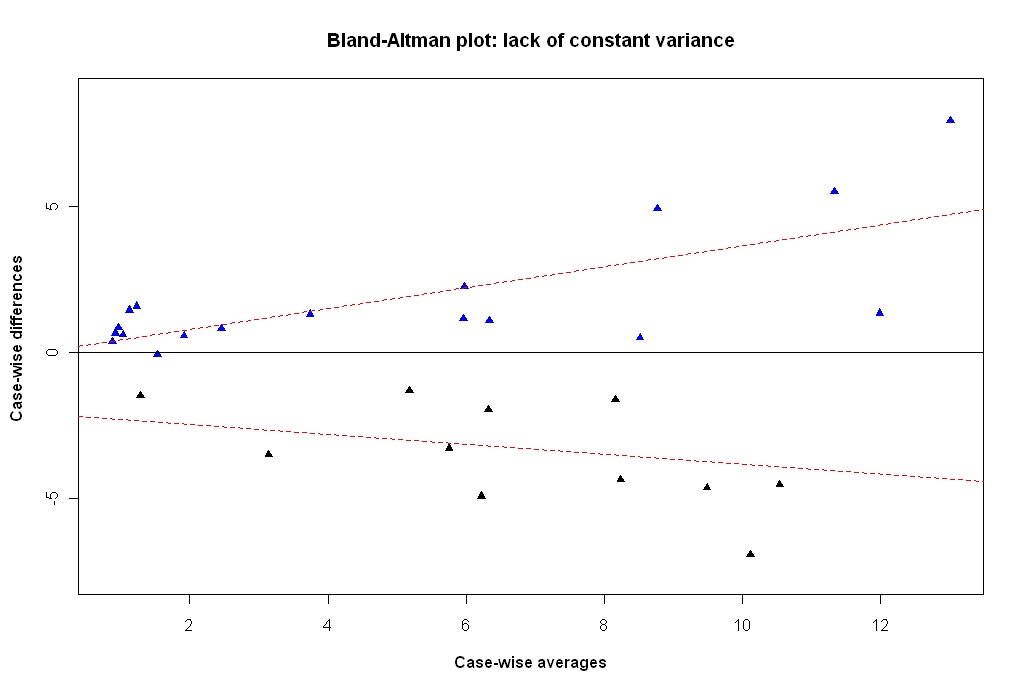
\includegraphics[height=90mm]{images/BAFanEffect.jpeg}
			\caption{Bland-Altman plot demonstrating the increase of variance over the range.}\label{BAFanEffect}
		\end{center}
	\end{figure}
	
	\begin{figure}[h!]
		\begin{center}
			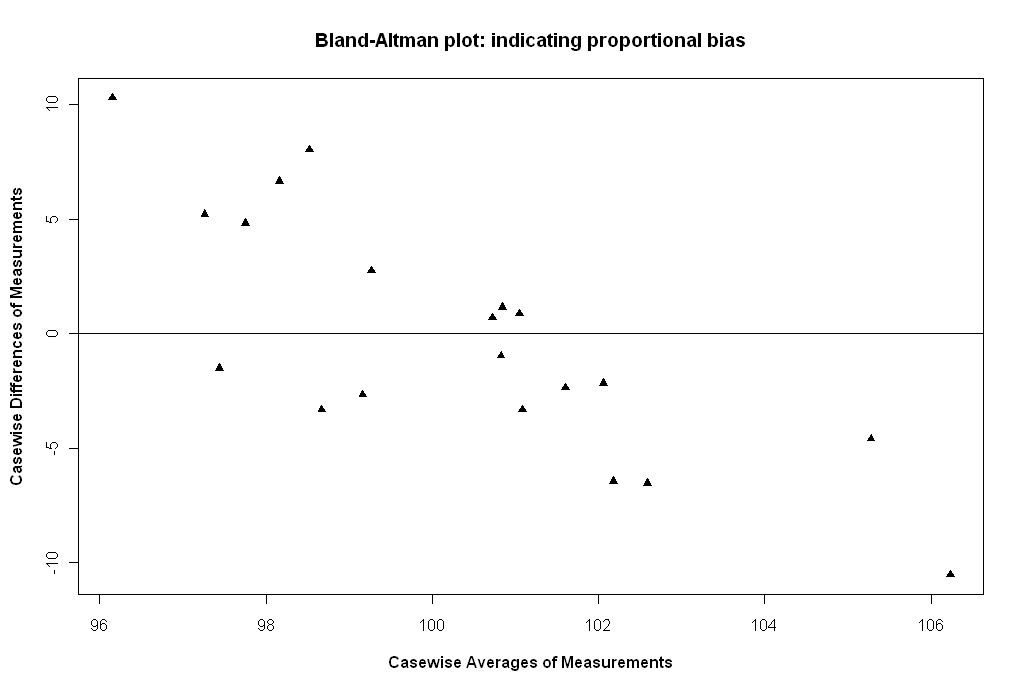
\includegraphics[height=90mm]{images/PropBias.jpeg}
			\caption{Bland-Altman plot indicating the presence of proportional bias.}\label{PropBias}
		\end{center}
	\end{figure}
	
	\begin{figure}[h!]
		\begin{center}
			\includegraphics[width=125mm]{images/BAOutliers.jpeg}
			\caption{Bland-Altman plot indicating the presence of potential outliers.}\label{Outliers}
		\end{center}
	\end{figure}
	
	\newpage
	
	
	The Bland-Altman plot also can be used to identify outliers. An
	outlier is an observation that is conspicuously different from the
	rest of the data that it arouses suspicion that it occurs due to a
	mechanism, or conditions, different to that of the rest of the
	observations. \citet*{BA99} do not recommend excluding outliers from analyzes,
	but remark that recalculation of the inter-method bias estimate,
	and further calculations based upon that estimate, are useful for
	assessing the influence of outliers. The authors remark that `we
	usually find that this method of analysis is not too sensitive to
	one or two large outlying differences'. Figure 1.6 demonstrates how the Bland-Altman
	plot can be used to visually inspect the presence of potential
	outliers.
	
	As a complement to the Bland-Altman plot, \citet{Bartko} proposes
	the use of a bivariate confidence ellipse, constructed for a
	predetermined level. \citet{AltmanEllipse} provides the relevant calculations for the
	ellipse. This ellipse is intended as a visual
	guidelines for the scatter plot, for detecting outliers and to
	assess the within- and between-subject variances.
	
	The minor axis relates to the between subject variability, whereas
	the major axis relates to the error mean square, with the ellipse
	depicting the size of both relative to each other.
	Consequently Bartko's ellipse provides a visual aid to determining the
	relationship between variances. If $\mbox{var}(a)$ is greater than $\mbox{var}(d)$, the orientation of the ellipse is horizontal. Conversely if $\mbox{var}(a)$ is less than $\mbox{var}(d)$, the orientation of the ellipse is vertical.
	
	
	%(Furthermore \citet{Bartko}
	%proposes formal testing procedures, that shall be discussed in due
	%course.)
	
	The Bland-Altman plot for the Grubbs data, complemented by Bartko's ellipse, is depicted in Figure 1.7.
	The fourth observation is shown to be outside the bounds of the ellipse, indicating that it is a potential outlier.
	
	
	\begin{figure}[h!]
		% Requires \usepackage{graphicx}
		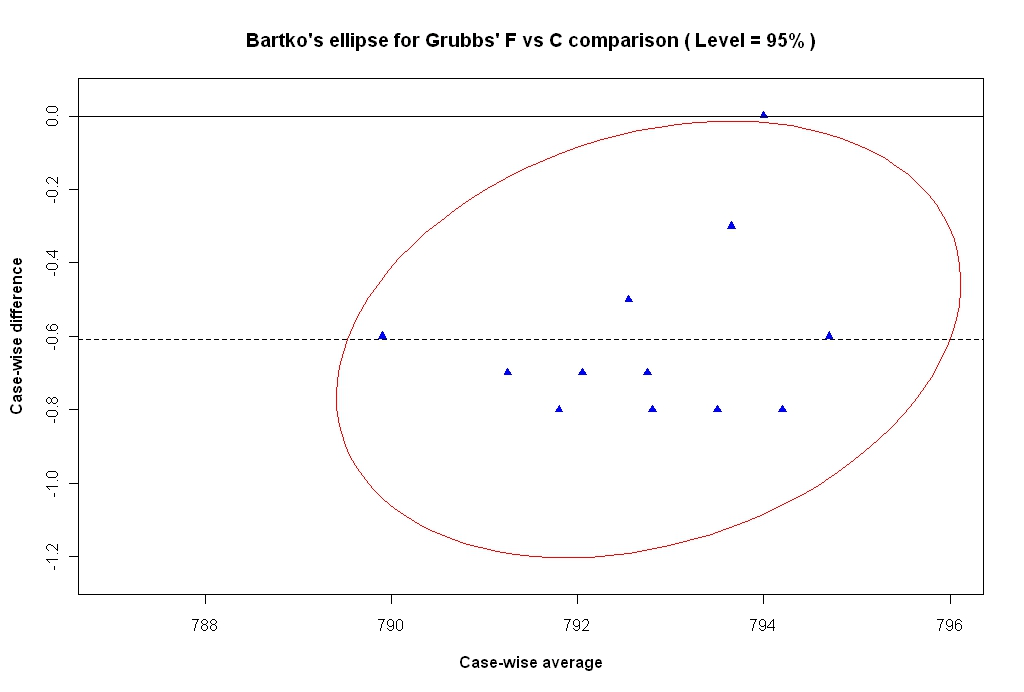
\includegraphics[width=130mm]{images/GrubbsBartko.jpeg}
		\caption{Bartko's Ellipse For Grubbs' Data.}\label{GrubbsBartko}
	\end{figure}
	
	The limitations of using bivariate approaches to outlier detection
	in the Bland-Altman plot can demonstrated using Bartko's ellipse.
	A covariate is added to the `F vs C' comparison that has a
	difference value equal to the inter-method bias, and an average
	value that markedly deviates from the rest of the average values
	in the comparison, i.e. 786. Table 1.8 depicts a $95\%$ confidence
	ellipse for this manipulated data set. By inspection of the
	confidence interval, a conclusion would be reached that this extra
	covariate is an outlier, in spite of the fact that this
	observation is wholly consistent with the conclusion of the
	Bland-Altman plot.
	
	\begin{figure}[h!]
		% Requires \usepackage{graphicx}
		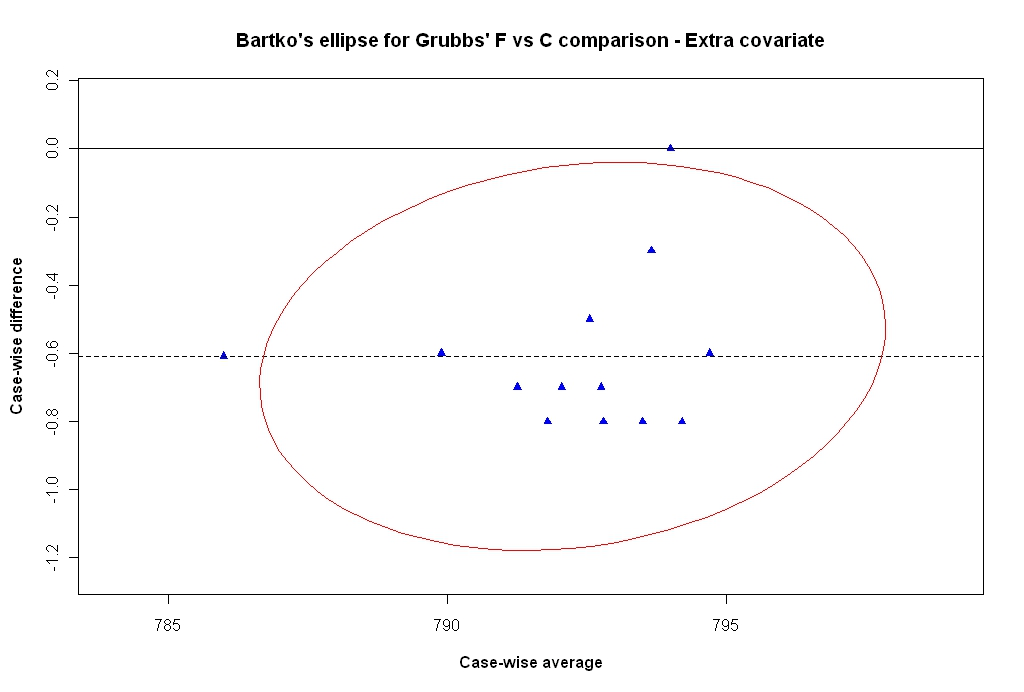
\includegraphics[width=130mm]{images/GrubbsBartko2.jpeg}
		\caption{Bartko's Ellipse For Grubbs' Data, with an extra covariate.}\label{GrubbsBartko2}
	\end{figure}
	
	
	Importantly, outlier classification must be informed by the logic of the
	data's formulation. In the Bland-Altman plot, the horizontal displacement of any
	observation is supported by two independent measurements. Any
	observation should not be considered an outlier on the basis of a
	noticeable horizontal displacement from the main cluster, as in
	the case with the extra covariate. Conversely, the fourth
	observation, from the original data set, should be considered an
	outlier, as it has a noticeable vertical displacement from the
	rest of the observations.
	
	%Grubbs' test is a statistical test used for detecting outliers in a
	%univariate data set that is assumed to be normally distributed.
	
	%\citet{Grubbs} defined an outlier as a co-variate that appears to
	%deviate markedly from other members of the sample in which it
	%occurs.
	
	In classifying whether a observation from a univariate data set is
	an outlier, many formal tests are available, such as the Grubbs test for outliers. In assessing
	whether a covariate in a Bland-Altman plot is an outlier, this
	test is useful when applied to the case-wise difference values treated as a
	univariate data set. The null hypothesis of the Grubbs test procedure is the absence
	of any outliers in the data set. Conversely, the alternative hypotheses is that there is at least one outlier
	present.
	
	The test statistic for the Grubbs test ($G$) is the largest
	absolute deviation from the sample mean divided by the standard
	deviation of the differences,
	\[
	G =  \displaystyle\max_{i=1,\ldots, n}\frac{\left \vert d_i -
		\bar{d}\right\vert}{S_{d}}.
	\]
	
	For the `F vs C' comparison it is the fourth observation gives
	rise to the test statistic, $G = 3.64$. The critical value is
	calculated using Student's $t$ distribution and the sample size,
	\[
	U = \frac{n-1}{\sqrt{n}} \sqrt{\frac{t_{\alpha/(2n),n-2}^2}{n - 2
			+ t_{\alpha/(2n),n-2}^2}}.
	\]
	For this test $U = 0.75$. The conclusion of this test is that the fourth observation in the `F vs C' comparison is an outlier, with $p-$value = 0.003, according with the previous result using Bartko's ellipse.
	
	\newpage
	
	

	\subsection{Adverse features}
	
	Estimates for inter-method bias and variance of differences are only meaningful if there is uniform inter-bias and variability throughout the range of measurements. Fulfilment of these assumptions can be checked by visual inspection of the plot.The prototype Bland-Altman plots depicted in Figures 1.4, 1.5 and 1.6 are derived from simulated data, for the purpose of demonstrating how the plot would inform an analyst of features that would adversely affect use of the recommended approach.
	
	Figure 1.4 demonstrates how the Bland-Altman plot would indicate
	increasing variance of differences over the measurement range.
	Fitted regression lines, for both the upper and lower half of the
	plot, has been added to indicate the trend. Figure 1.5 is an
	example of cases where the inter-method bias changes over the
	measurement range. This is known as proportional bias, and is
	defined by \citet{ludbrook97} as meaning that `one method gives
	values that are higher (or lower) than those from the other by an
	amount that is proportional to the level of the measured
	variable'. In both Figures 1.4 and 1.5, the assumptions necessary
	for further analysis using the limits of agreement are violated.
	
	Application of regression techniques to the Bland-Altman plot, and
	subsequent formal testing for the constant variability of
	differences is informative. The data set may be divided into two
	subsets, containing the observations wherein the difference values
	are less than and greater than the inter-method bias respectively.
	For both of these fits, hypothesis tests for the respective slopes
	can be performed. While both tests could be considered separately,
	multiple comparison procedures, such as the Benjamini-Hochberg
	\citep{BH} test, are advisable.
	
	\begin{figure}[h!]
		\begin{center}
			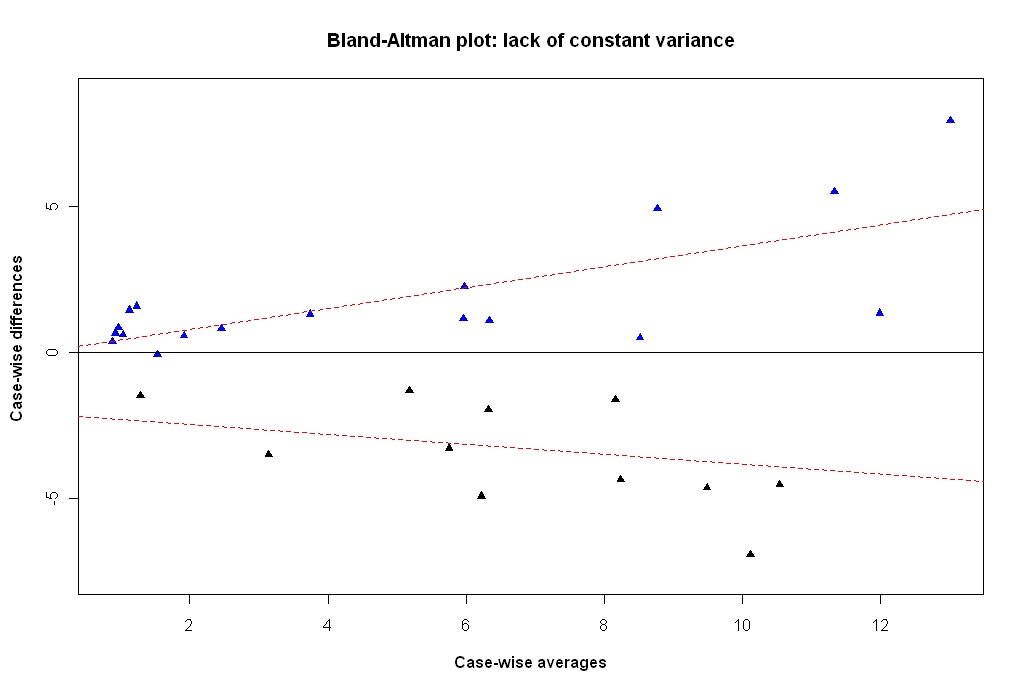
\includegraphics[height=90mm]{images/BAFanEffect.jpeg}
			\caption{Bland-Altman plot demonstrating the increase of variance over the range.}\label{BAFanEffect}
		\end{center}
	\end{figure}
	
	\begin{figure}[h!]
		\begin{center}
			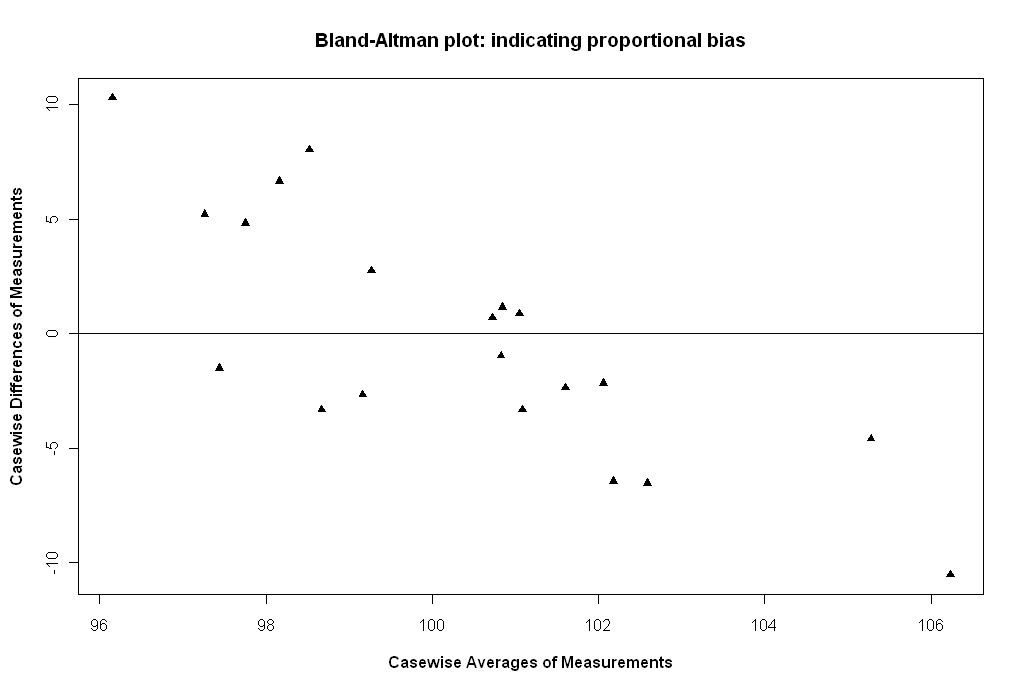
\includegraphics[height=90mm]{images/PropBias.jpeg}
			\caption{Bland-Altman plot indicating the presence of proportional bias.}\label{PropBias}
		\end{center}
	\end{figure}
	
	\begin{figure}[h!]
		\begin{center}
			\includegraphics[width=125mm]{images/BAOutliers.jpeg}
			\caption{Bland-Altman plot indicating the presence of potential outliers.}\label{Outliers}
		\end{center}
	\end{figure}
	
	\newpage
	
	
	The Bland-Altman plot also can be used to identify outliers. An
	outlier is an observation that is conspicuously different from the
	rest of the data that it arouses suspicion that it occurs due to a
	mechanism, or conditions, different to that of the rest of the
	observations. \citet*{BA99} do not recommend excluding outliers from analyses,
	but remark that recalculation of the inter-method bias estimate,
	and further calculations based upon that estimate, are useful for
	assessing the influence of outliers. The authors remark that `we
	usually find that this method of analysis is not too sensitive to
	one or two large outlying differences'. Figure 1.6 demonstrates how the Bland-Altman
	plot can be used to visually inspect the presence of potential
	outliers.
	
	As a complement to the Bland-Altman plot, \citet{Bartko} proposes
	the use of a bivariate confidence ellipse, constructed for a
	predetermined level. \citet{AltmanEllipse} provides the relevant calculations for the
	ellipse. This ellipse is intended as a visual
	guidelines for the scatter plot, for detecting outliers and to
	assess the within- and between-subject variances.
	
	The minor axis relates to the between subject variability, whereas
	the major axis relates to the error mean square, with the ellipse
	depicting the size of both relative to each other.
	Consequently Bartko's ellipse provides a visual aid to determining the
	relationship between variances. If $\mbox{var}(a)$ is greater than $\mbox{var}(d)$, the orientation of the ellipse is horizontal. Conversely if $\mbox{var}(a)$ is less than $\mbox{var}(d)$, the orientation of the ellipse is vertical.
	
	
	%(Furthermore \citet{Bartko}
	%proposes formal testing procedures, that shall be discussed in due
	%course.)
	
	The Bland-Altman plot for the Grubbs data, complemented by Bartko's ellipse, is depicted in Figure 1.7.
	The fourth observation is shown to be outside the bounds of the ellipse, indicating that it is a potential outlier.
	
	
	\begin{figure}[h!]
		% Requires \usepackage{graphicx}
		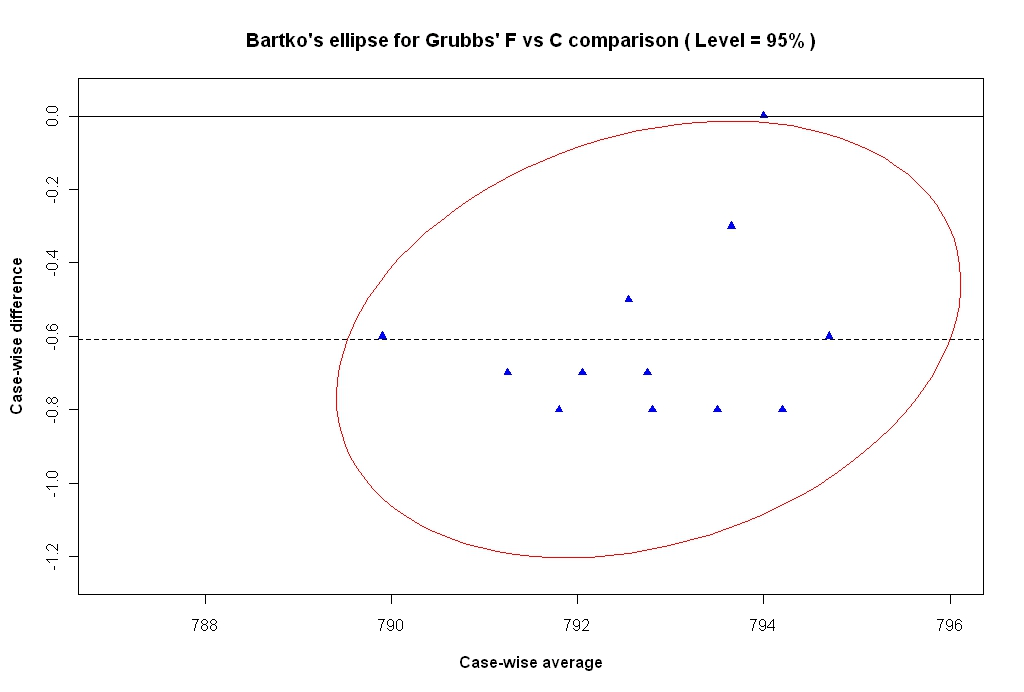
\includegraphics[width=130mm]{images/GrubbsBartko.jpeg}
		\caption{Bartko's Ellipse for Grubbs' data.}\label{GrubbsBartko}
	\end{figure}
	
	The limitations of using bivariate approaches to outlier detection
	in the Bland-Altman plot can demonstrated using Bartko's ellipse.
	A covariate is added to the `F vs C' comparison that has a
	difference value equal to the inter-method bias, and an average
	value that markedly deviates from the rest of the average values
	in the comparison, i.e. 786. Table 1.8 depicts a $95\%$ confidence
	ellipse for this manipulated data set. By inspection of the
	confidence interval, we would conclude that this extra
	covariate is an outlier, in spite of the fact that this
	observation is very close to the inter-method bias as determined by this approach.
	
	\begin{figure}[h!]
		% Requires \usepackage{graphicx}
		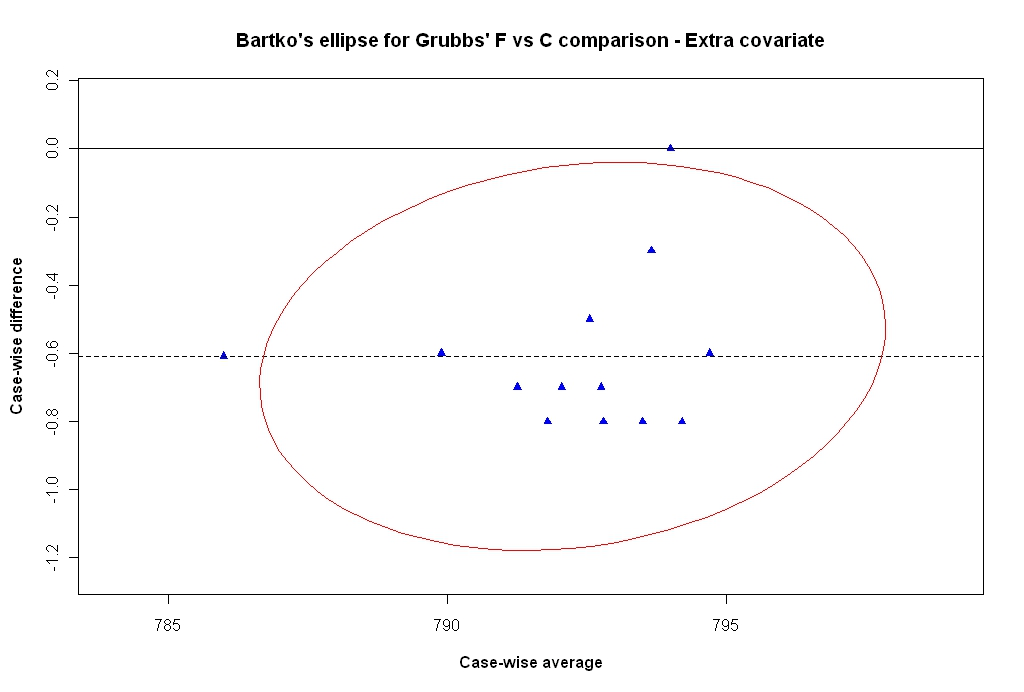
\includegraphics[width=130mm]{images/GrubbsBartko2.jpeg}
		\caption{Bartko's Ellipse for Grubbs' data, with an extra covariate.}\label{GrubbsBartko2}
	\end{figure}
	
	
	Importantly, outlier classification must be informed by the logic of the
	mechanism that produces the data. In the Bland-Altman plot, the horizontal displacement (i.e. the average) of any
	observation is supported by two separate measurements. Any
	observation should not be considered an outlier on the basis of a
	noticeable horizontal displacement from the main cluster, as in
	the case with the extra covariate. Conversely, the fourth
	observation, from the original data set, should be considered an
	outlier, as it has a noticeable vertical displacement from the
	rest of the observations.
	
	%Grubbs' test is a statistical test used for detecting outliers in a
	%univariate data set that is assumed to be normally distributed.
	
	%\citet{Grubbs} defined an outlier as a co-variate that appears to
	%deviate markedly from other members of the sample in which it
	%occurs.
	
	In classifying whether a observation from a univariate data set is
	an outlier, many formal tests are available, such as the Grubbs test for outliers. In assessing
	whether a covariate in a Bland-Altman plot is an outlier, this
	test is useful when applied to the case-wise difference values treated as a
	univariate data set. The null hypothesis of the Grubbs test procedure is the absence
	of any outliers in the data set. Conversely, the alternative hypotheses is that there is at least one outlier
	present.
	
	The test statistic for the Grubbs test ($G$) is the largest
	absolute deviation from the sample mean divided by the standard
	deviation of the differences,
	\[
	G =  \displaystyle\max_{i=1,\ldots, n}\frac{\left \vert d_i -
		\bar{d}\right\vert}{S_{d}}.
	\]
	
	For the `F vs C' comparison it is the fourth observation gives
	rise to the test statistic, $G = 3.64$. The critical value is
	calculated using Student's $t$ distribution and the sample size,
	\[
	U = \frac{n-1}{\sqrt{n}} \sqrt{\frac{t_{\alpha/(2n),n-2}^2}{n - 2
			+ t_{\alpha/(2n),n-2}^2}}.
	\]
	For this test $U = 0.75$. The conclusion of this test is that the fourth observation in the `F vs C' comparison is an outlier, with $p-$value = 0.003, in accordance with the previous result of Bartko's ellipse.
	
\newpage	

\subsection{Adverse features}

Estimates for inter-method bias and variance of differences are only meaningful if there is uniform inter-bias and variability throughout the range of measurements. Fulfilment of these assumptions can be checked by visual inspection of the plot.The prototype Bland-Altman plots depicted in Figures 1.4, 1.5 and 1.6 are derived from simulated data, for the purpose of demonstrating how the plot would inform an analyst of features that would adversely affect use of the recommended methodology.

Figure 1.4 demonstrates how the Bland-Altman plot would indicate increasing variance of differences over the measurement range.
Fitted regression lines, for both the upper and lower half of the plot, has been added to indicate the trend. Figure 1.5 is an
example of cases where the inter-method bias changes over the measurement range. This is known as proportional bias, and is defined by \citet{ludbrook97} as meaning that `one method gives values that are higher (or lower) than those from the other by an
amount that is proportional to the level of the measured
variable'. In both Figures 1.4 and 1.5, the assumptions necessary
for further analysis using the limits of agreement are violated.

Application of regression techniques to the Bland-Altman plot, and subsequent formal testing for the constant variability of
differences is informative. The data set may be divided into two subsets, containing the observations wherein the difference values
are less than and greater than the inter-method bias respectively. For both of these fits, hypothesis tests for the respective slopes
can be performed. While both tests can be considered separately, multiple comparison procedures, such as the Benjamini-Hochberg
\citep{BH} test, should be also be used.

\begin{figure}[h!]
	\begin{center}
		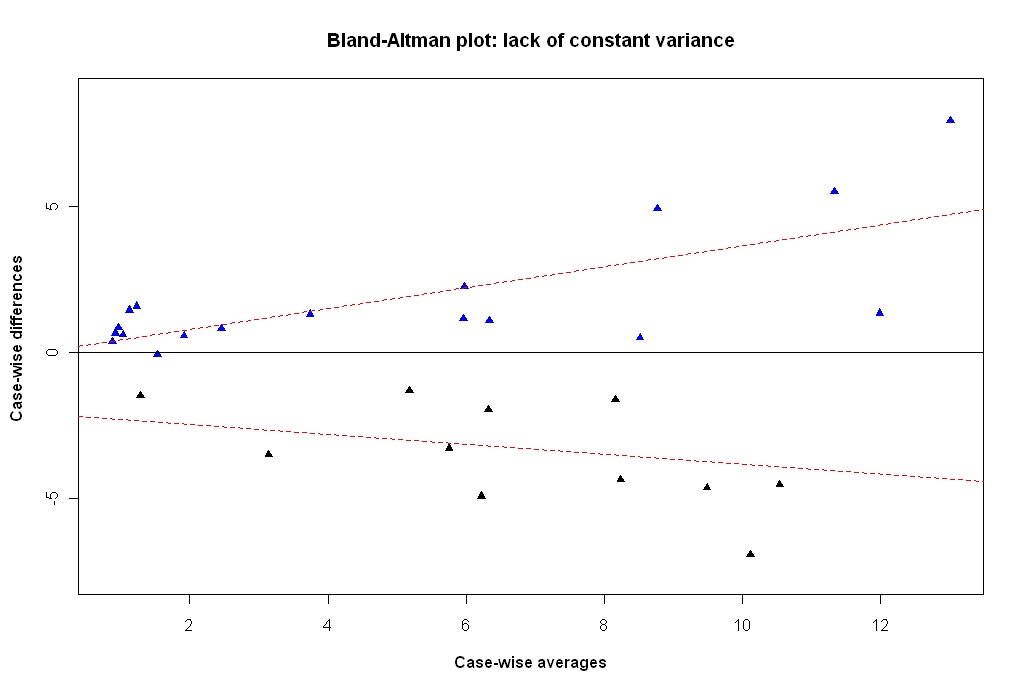
\includegraphics[height=90mm]{images/BAFanEffect.jpeg}
		\caption{Bland-Altman plot demonstrating the increase of variance over the range.}\label{BAFanEffect}
	\end{center}
\end{figure}

\begin{figure}[h!]
	\begin{center}
		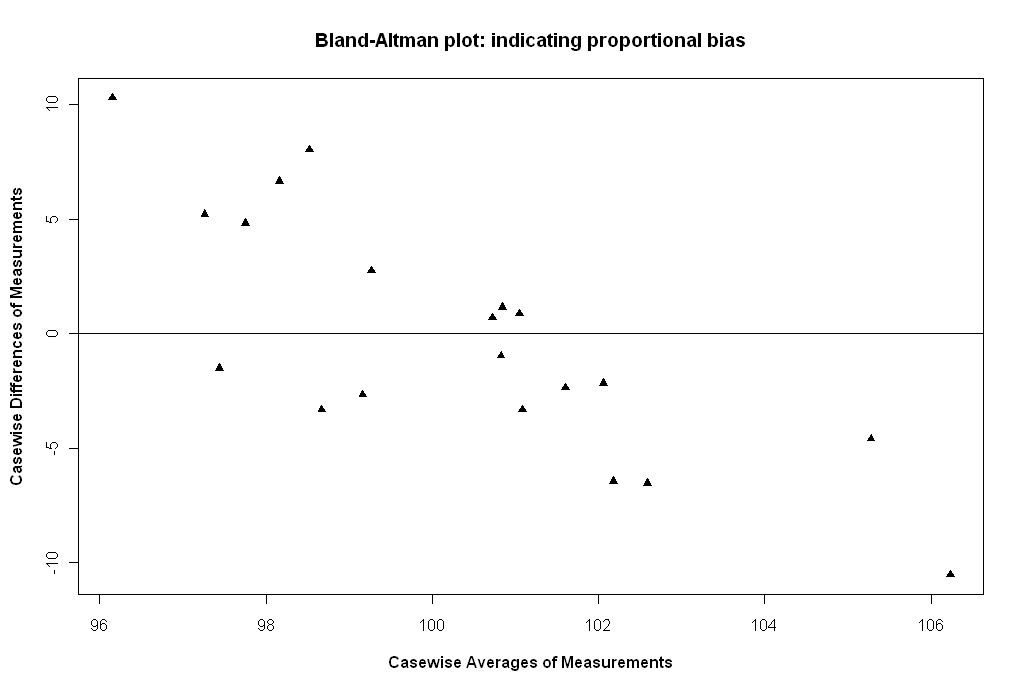
\includegraphics[height=90mm]{images/PropBias.jpeg}
		\caption{Bland-Altman plot indicating the presence of proportional bias.}\label{PropBias}
	\end{center}
\end{figure}

\begin{figure}[h!]
	\begin{center}
		\includegraphics[width=125mm]{images/BAOutliers.jpeg}
		\caption{Bland-Altman plot indicating the presence of potential outliers.}\label{Outliers}
	\end{center}
\end{figure}



The Bland-Altman plot also can be used to identify outliers. An outlier is an observation that is conspicuously different from the
rest of the data that it arouses suspicion that it occurs due to a mechanism, or conditions, different to that of the rest of the
observations. \citet*{BA99} do not recommend excluding outliers from analyzes, but remark that recalculation of the inter-method bias estimate, and further calculations based upon that estimate, are useful for assessing the influence of outliers. The authors remark that `we usually find that this method of analysis is not too sensitive to one or two large outlying differences'. Figure 1.6 demonstrates how the Bland-Altman plot can be used to visually inspect the presence of potential outliers.

\newpage
	\section{Bland-Altman Approach}
	The issue of whether two measurement methods comparable to the
	extent that they can be used interchangeably with sufficient
	accuracy is encountered frequently in scientific research.
	Historically, comparison of two methods of measurement was carried
	out by use of paired sample $t-$test, correlation coefficients or
	simple linear regression. However, simple linear regression is unsuitable for method comparison studies due to the assumption that one variable is measured without error. In comparing two methods, both methods are assume to have attendant random error.
	
	\citet{BA83} highlighted the inadequacies of these approaches for comparing two methods of measurement, and proposed methodologies with this specific application in mind. Although the authors also acknowledge the opportunity to apply other, more complex, approaches, but argue that simpler approaches is preferable, especially when the
	results must be `explained to non-statisticians'.
	
	Notwithstanding previous remarks about linear regression, the first step recommended, which the authors argue should be mandatory, is the construction of a scatter plot of the data. Scatterplots can facilitate an initial judgement and
	helping to identify potential outliers, with the addition of the line of equality. In the case of good agreement, the observations would be distributed closely along this line. However, they are not useful for a thorough examination of the data. \citet{BritHypSoc} notes that
	data points will tend to cluster around the line of equality, obscuring interpretation.
	
	
	A scatter plot of the Grubbs data is shown in Figure 1.1. Visual inspection confirms the previous conclusion that inter-method bias is present, i.e. the Fotobalk device has a tendency to record a lower velocity.
	
	\begin{figure}[h!]
		\begin{center}
			\includegraphics[width=125mm]{images/GrubbsScatter.jpeg}
			\caption{Scatter plot for Fotobalk and Counter methods.}\label{GrubbsScatter}
		\end{center}
	\end{figure}
	
	\citet{Dewitte} notes that scatter plots were very seldom
	presented in the Annals of Clinical Biochemistry. This apparently
	results from the fact that the `Instructions for Authors' dissuade
	the use of regression analysis, which conventionally is
	accompanied by a scatter plot.
	
	\newpage




	\section{Blackwood Bradley Model} 
	
	\citet{BB89} have developed a regression based procedure for
	assessing the agreement. This approach performs a simultaneous test for the equivalence of
	means and variances of the respective methods. Using simple linear
	regression of the differences of each pair against the sums, a
	line is fitted to the model, with estimates for intercept and
	slope ($\hat{\beta}_{0}$ and $\hat{\beta}_{1}$).
	%We have identified
	%this approach  to be examined to see if it can be used as a %foundation for a test perform a test on
	%means and variances individually.
	\begin{equation}
	D = (X_{1}-X_{2})
	\end{equation}
	\begin{equation}
	M = (X_{1} + X_{2}) /2
	\end{equation}
	The Bradley Blackwood Procedure fits D on M as follows:\\
	\begin{equation}
	D = \beta_{0} + \beta_{1}M
	\end{equation}
	This technique offers a formal simultaneous hypothesis test for the
	mean and variance of two paired data sets.  The null
	hypothesis of this test is that the mean ($\mu$) and variance
	($\sigma^{2}$) of both data sets are equal if the slope and
	intercept estimates are equal to zero(i.e $\sigma^{2}_{1} =
	\sigma^{2}_{2}$ and $\mu_{1}=\mu_{2}$ if and only if $\beta_{0}=
	\beta_{1}=0$ )
	
	A test statistic is then calculated from the regression analysis
	of variance values \citep{BB89} and is distributed as `$F$' random
	variable. The degrees of freedom are $\nu_{1}=2$ and $\nu_{1}=n-2$
	(where $n$ is the number of pairs). The critical value is chosen
	for $\alpha\%$ significance with those same degrees of freedom.
	\citet{Bartko} amends this approach for use in method
	comparison studies, using the averages of the pairs, as opposed to
	the sums, and their differences. This approach can facilitate
	simultaneous usage of test with the Bland-Altman approach.
	Bartko's test statistic take the form:
	\[ F.test = \frac{(\Sigma d^{2})-SSReg}{2MSReg}
	\]
	% latex table generated in R 2.6.0 by xtable 1.5-5 package
	% Mon Aug 31 15:53:51 2009
	\begin{table}[h!]
		\begin{center}
			\begin{tabular}{lrrrrr}
				\hline
				& Df & Sum Sq & Mean Sq & F value & Pr($>$F) \\
				\hline
				Averages & 1 & 0.04 & 0.04 & 0.74 & 0.4097 \\
				Residuals & 10 & 0.60 & 0.06 &  &  \\
				\hline
			\end{tabular}
			\caption{Regression ANOVA of case-wise differences and averages
				for Grubbs Data}
		\end{center}
	\end{table}
	%(calculate using R code $qf(0.95,2,10)$).
	
	For the Grubbs data, $\Sigma d^{2}=5.09 $, $SSReg = 0.60$ and
	$MSreg=0.06$ Therefore the test statistic is $37.42$, with a
	critical value of $4.10$. Hence the means and variance of the
	Fotobalk and Counter chronometers are assumed to be simultaneously
	equal.
	
	Importantly, this approach determines whether there is both
	inter-method bias and precision present, or alternatively if there
	is neither present. It has previously been demonstrated that there
	is a inter-method bias present, but as this procedure does not
	allow for separate testing, no conclusion can be drawn on the
	comparative precision of both methods.
	
	

\section{Bland-Altman methodology}
The issue of whether two measurement methods comparable to the extent that they can be used interchangeably with sufficient
accuracy is encountered frequently in scientific research. Historically comparison of two methods of measurement was carried out by use of paired sample $t-$test, correlation coefficients or simple linear regression. Simple linear regression is unsuitable for method comparison studies because of the required assumption that one variable is measured without error. In comparing two methods, both methods are assume to have attendant random error.
	
Statisticians Martin Bland and Douglas Altman recognized the inadequacies of these analyzes and articulated quite thoroughly the basis on which of which they are unsuitable for comparing two methods of measurement \citep*{BA83}. Furthermore they proposed their simple methodology specifically constructed for method comparison studies. They acknowledge the opportunity to apply other valid, but complex, methodologies, but argue that a simple approach is preferable, especially when the	results must be `explained to non-statisticians'.
	
Notwithstanding previous remarks about linear regression, the first step recommended, which the authors argue should be mandatory, is construction of a simple scatter plot of the data. The line of equality should also be shown, as it is necessary to give the correct interpretation of how both methods compare. In the case of good agreement, the observations would be distributed closely along the line of equality. A scatter plot of the Grubbs data is shown in Figure 1.1. Visual inspection confirms the previous conclusion that there is an inter-method bias present, i.e. Fotobalk device has a tendency to record a lower velocity.
	
	\begin{figure}[h!]
		\begin{center}
			\includegraphics[width=125mm]{images/GrubbsScatter.jpeg}
			\caption{Scatter plot For Fotobalk and Counter Methods.}\label{GrubbsScatter}
		\end{center}
	\end{figure}
	
\citet{Dewitte} notes that scatter plots were very seldom presented in the Annals of Clinical Biochemistry. This apparently results from the fact that the `Instructions for Authors' dissuade the use of regression analysis, which conventionally is accompanied by a scatter plot.
	


	
	
	\chapter{The Bland Altman Plot}

	\section{Bland Altman Plots}
	The issue of whether two measurement methods comparable to the
	extent that they can be used interchangeably with sufficient
	accuracy is encountered frequently in scientific research.
	Historically comparison of two methods of measurement was carried
	out by use of correlation coefficients or simple linear
	regression. Bland and Altman recognized the inadequacies of these
	analyses and articulated quite thoroughly the basis on which of
	which they are unsuitable for comparing two methods of measurement
	\citep*{BA83}.
	
	
	Furthermore they proposed their simple methodology specifically
	constructed for method comparison studies. They acknowledge that
	there are other valid, but complex, methodologies, and argue that
	a simple approach is preferable to this complex approaches,
	\emph{especially when the results must be explained to
		non-statisticians} \citep*{BA83}.
	
	\smallskip
	
	Notwithstanding previous remarks about regression, the first step
	recommended ,which the authors argue should be mandatory,is
	construction of a simple scatter plot of the data. The line of
	equality ($X=Y$) should also be shown, as it is necessary to give
	the correct interpretation of how both methods compare. A scatter
	plot of the Grubbs data is shown in figure 2.1. A visual
	inspection thereof confirms the previous conclusion that there is
	an inter method bias present, i.e. Fotobalk device has a tendency
	to record a lower velocity.
	
	\begin{figure}[h!]
		\begin{center}
			\includegraphics[width=130mm]{images/GrubbsScatter.jpeg}
			\caption{Scatter plot For Fotobalk and Counter Methods}\label{GrubbsScatter}
		\end{center}
	\end{figure}
	
	In light of shortcomings associated with scatterplots,
	\citet*{BA83} recommend a further analysis of the data. Firstly
	differences of measurements of two methods on the same subject
	should  be calculated, and then the average of those measurements
	(Table 2.1). These differences and averages are then plotted
	(Figure 2.2).
	
	
	
	
	The dashed line in Figure 2.2 alludes to the inter method bias
	between the two methods, as mentioned previously. Bland and Altman
	recommend the estimation of inter method bias by calculating the
	average of the differences. In the case of Grubbs data the inter
	method bias is $-0.6083$ metres per second.
	\newpage
	
	% latex table generated in R 2.6.0 by xtable 1.5-5 package
	% Thu Aug 27 16:31:52 2009
	\begin{table}[tbh]
		\begin{center}
			
			\begin{tabular}{rrrrr}
				\hline
				Round & Fotobalk [F] & Counter [C] & Differences [F-C] & Averages [(F+C)/2] \\
				\hline
				1 & 793.80 & 794.60 & -0.80 & 794.20 \\
				2 & 793.10 & 793.90 & -0.80 & 793.50 \\
				3 & 792.40 & 793.20 & -0.80 & 792.80 \\
				4 & 794.00 & 794.00 & 0.00 & 794.00 \\
				5 & 791.40 & 792.20 & -0.80 & 791.80 \\
				6 & 792.40 & 793.10 & -0.70 & 792.80 \\
				7 & 791.70 & 792.40 & -0.70 & 792.00 \\
				8 & 792.30 & 792.80 & -0.50 & 792.50 \\
				9 & 789.60 & 790.20 & -0.60 & 789.90 \\
				10 & 794.40 & 795.00 & -0.60 & 794.70 \\
				11 & 790.90 & 791.60 & -0.70 & 791.20 \\
				12 & 793.50 & 793.80 & -0.30 & 793.60 \\
				\hline
			\end{tabular}
			\caption{Fotobalk and Counter Methods: Differences and Averages}
		\end{center}
	\end{table}
	
	
	\begin{figure}[h!]
		\begin{center}
			\includegraphics[width=120mm]{images/GrubbsBAplot.jpeg}
			\caption{Bland Altman Plot For Fotobalk and Counter Methods}\label{GrubbsBA}
		\end{center}
	\end{figure}
	
	\newpage
	By inspection of the plot, it is also possible to compare the precision of each method. Noticeably the differences tend to
	increase as the averages increase.
	
	\subsection{Inspecting the Data}
	Bland-Altman plots are a powerful graphical methodology for making a visual assessment of the data. \citet*{BA83} express the motivation for this plot thusly:
	\begin{quote}
		"From this type of plot it is much easier to assess the magnitude
		of disagreement (both error and bias), spot outliers, and see
		whether there is any trend, for example an increase in
		(difference) for high values. This way of plotting the data is a
		very powerful way of displaying the results of a method comparison
		study."
	\end{quote}
	
	
	Figures 1.3 1.4 and 1.5 are three Bland-Altman plots derived from
	simulated data, each for the purpose of demonstrating how the plot
	would inform an analyst of trends that would adversely affect use
	of the recommended methodology. Figure 1.3 demonstrates how the
	Bland Altman plot would indicate increasing variance of
	differences over the measurement range. Figure 1.4 is an example
	of cases where the inter-method bias changes over the measurement
	range. This is known as proportional bias \citep{ludbrook97}.
	
	
	\begin{figure}[h!]
		\begin{center}
			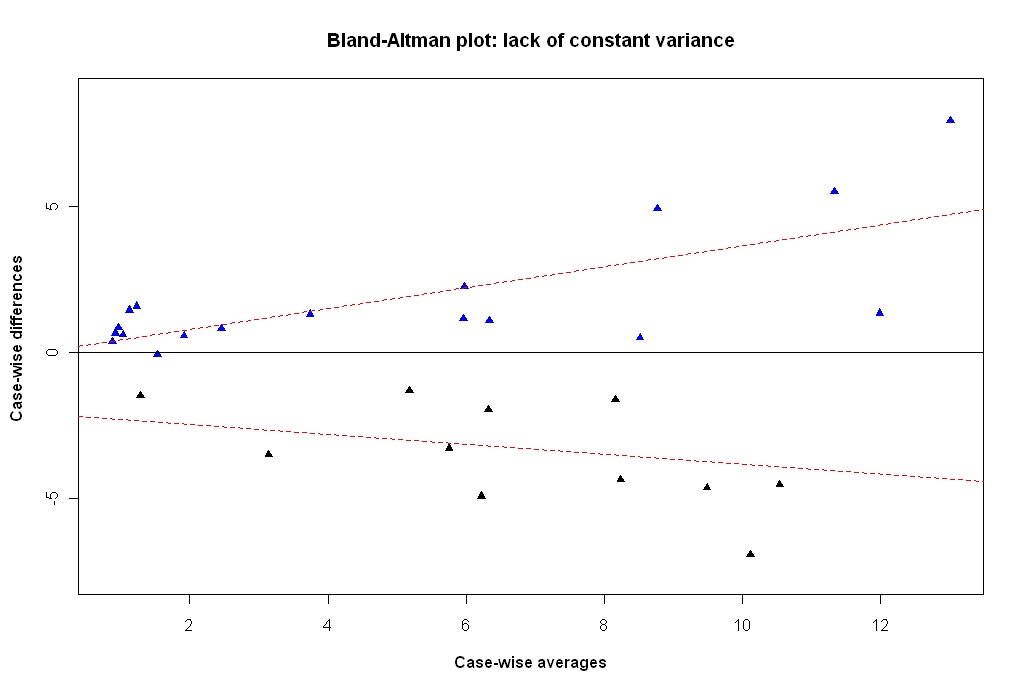
\includegraphics[width=125mm]{images/BAFanEffect.jpeg}
			\caption{Bland-Altman Plot demonstrating the increase of variance over the range}\label{BAFanEffect}
		\end{center}
	\end{figure}
	
	\begin{figure}[h!]
		\begin{center}
			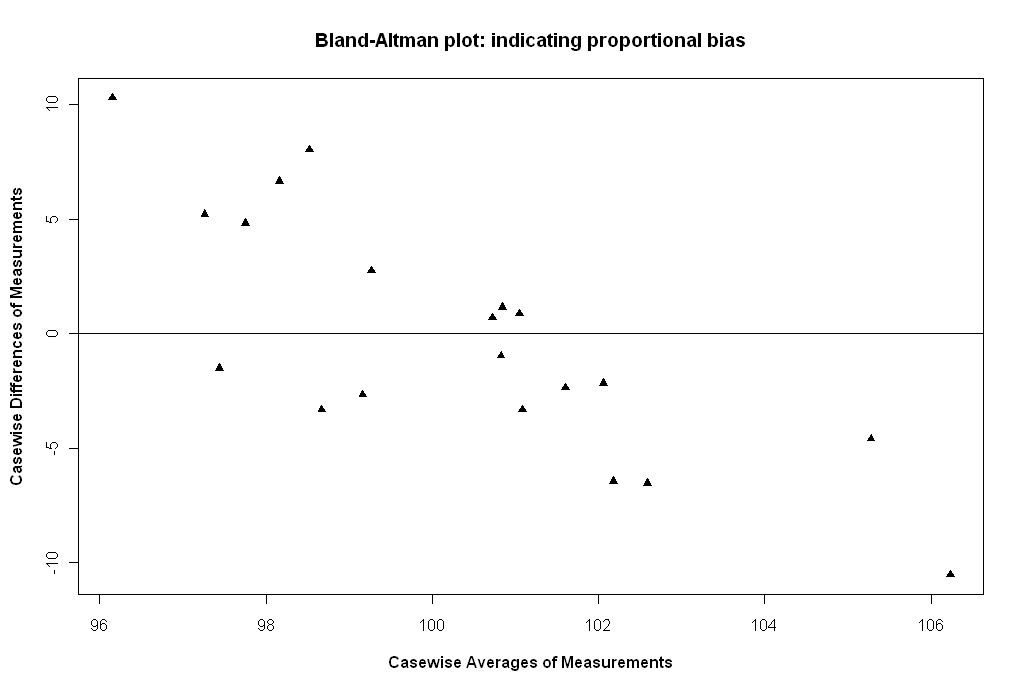
\includegraphics[width=125mm]{images/PropBias.jpeg}
			\caption{Bland-Altman Plot indicating the presence of proportional bias}\label{PropBias}
		\end{center}
	\end{figure}
	
	\newpage
	Figure 1.4 is an example of cases where the inter-method bias
	changes over the measurement range. This is known as\textit{ proportional
		bias} (Ludbrook, 1997). Both of these cases violate the assumptions
	necessary for further analysis using limits of agreement ,which
	shall be discussed later. The plot also can be used to identify
	outliers. An outlier is an observation that is numerically distant
	from the rest of the data. Classification thereof is a subjective
	decision in any analysis, but must be informed by the logic of the
	formulation. Figure 1.5 is a Bland Altman plot with two
	conspicuous observations, at the extreme left and right of the
	plot respectively.
	
	
	%\begin{figure}[h!]
	%	\begin{center}
	%		\includegraphics[width=125mm]{BAOutliers.jpeg}
	%		\caption{Bland-Altman Plot indicating the presence of Outliers}\label{PropBias}
	%	\end{center}
	%\end{figure}
	
	In the Bland-Altman plot, the horizontal displacement of any
	observation is supported by two independent measurements. Hence
	any observation , such as the one on the extreme right of figure
	1.5, should not be considered an outlier on the basis of a
	noticeable horizontal displacement from the main cluster. The one
	on the extreme left should be considered an outlier, as it has a
	noticeable vertical displacement from the rest of the
	observations.
	
	\citet*{BA99} do not recommend excluding outliers from analyses.
	However recalculation of the inter-method bias estimate , and
	further calculations based upon that estimate, are useful for
	assessing the influence of outliers.\citep{BA99} states that
	\emph{"We usually find that this method of analysis is not too
		sensitive to one or two large outlying differences."}
	
	\subsection{Limits of Agreement}
	\citet{BA86} introduces an elaboration of the plot, adding to the
	plot `limits of agreement' to the plot. These limits are based
	upon the standard deviation of the differences. The discussion
	shall be reverted to these limits of agreement in due course.
	

	\subsection{Agreement} Bland and Altman (1986) defined perfect
	agreement as the case where all of the pairs of rater data lie
	along the line of equality, where the line of equality is defined
	as the $45$ degree line passing through the origin(i.e. the $X=Y$
	line).
	
	Bland and Altman (1986)expressed this in the terms \emph{we want
		to know by how much the new method is likely to differ from the
		old; if this is not enough to cause problems in clinical
		interpretation we can replace the old method by the new or use the
		two interchangeably. How far apart measurements can be without
		causing difficulties will be a question of judgment. Ideally, it
		should be defined in advance to help in the interpretation of the
		method comparisonand to choose the sample size” .}
	%----------------------------------------------------------------------------%
	\subsection{Bias}
	Bland and Altman define bias a \emph{a consistent tendency for one
		method to exceed the other} and propose estimating its value
	by determining the mean of the differences. The variation about
	this mean shall be estimated by the  standard deviation of the
	differences. Bland and Altman remark that these estimates are based on the
	assumption that bias and variability are constant throughout the
	range of measures.

	
	%----------------------------------------------------------------------------%
	\subsection{Bland Altman Plot}
	Bland Altman have recommended the use of graphical techniques to
	assess agreement. Principally their method is calculating , for
	each pair of corresponding two methods of measurement of some
	underlying quantity, with no replicate measurements, the
	difference and mean. Differences are then plotted against the
	mean.
	
	\textbf{\textit{Hopkins}} argued that the bias in a subsequent Bland-Altman plot was
	due, in part, to using least-squares regression at the calibration
	phase.
	
	
	%This page also shows the standard deviation (SD) of the
	%differences between the two assay methods. The SD value is used to
	%calculate the limits of agreement, computed as the mean bias plus
	%or minus 1.96 times its SD.
	%----------------------------------------------------------------------------%
	\subsection{The Bland Altman Plot}
	In 1986 Bland and Altman published a paper in the Lancet proposing
	the difference plot for use for method comparison purposes. It has
	proved highly popular ever since. This is a simple, and widely
	used , plot of the differences of each data pair, and the
	corresponding average value. An important requirement is that the
	two measurement methods use the same scale of measurement.
	
	\subsubsection{scatter plots} The authors advise the
	use of scatter plots to identify outliers, and to determine if
	there is curvilinearity present. In the region of linearity
	,simple linear regression may yield results of interest.
	
	\subsection{Effect of Outliers} Another argument against
	the use of model I regression is based on outliers. Outliers can
	adversely influence the fitting of a regression model. Cornbleet
	and Cochrane compare a regression model influenced by an outlier
	with a model for the same data set, with the outlier excluded from
	the data set. A demonstration of the effect of outliers was made
	in Bland Altman's 1986 paper. However they discourage the
	exclusion of outliers.
	
	%----------------------------------------------------------------------------%
\section{Bland Altman Plot} Bland Altman have
	recommended the use of graphical techniques to assess agreement.
	Principally their method is calculating , for each pair of
	corresponding two methods of measurement of some underlying
	quantity, with no replicate measurements, the difference and mean.
	Differences are then plotted against the mean.
	
	
	Hopkins argued that the bias in a subsequent Bland-Altman plot was
	due, in part, to using least-squares regression at the calibration
	phase.
	
	\subsection{Bland Altman plots using 'Gold Standard' raters}
	According to Bland and Altman, one should use the methodology
	previous outlined, even when one of the raters is a Gold Standard.
	
	
	\subsection{Bias Detection}
	further to this method, the presence of constant bias may be
	indicated if the average value differences is not equal to zero.
	Bland and Altman does, however, indicate the indication of absence
	of bias does not provide sufficient information to allow a
	judgement as to whether or not one method can be substituted for
	another.
	
	
	
	
	\subsection{Limits Of Agreement}
	Bland and Altman proposed a pair of Limits of agreement. These
	limits are intended to demonstrate the range in which 95\% of the
	sample data should lie. The Limits of agreement centre on the
	average difference line and are 1.96 times the standard deviation
	above and below the average difference line.
	\\
	How this relates the overall population is unclear. It seems that
	it depends on an expert to decide whether or not the range of
	differences is acceptable. In a study A Bland-Altman plots compare
	two assay methods. It plots the difference between the two
	measurements on the Y axis, and the average of the two
	measurements on the X axis
	
	% introduces
	A third element of the Bland-Altman methodology, an interval known
	as `limits of agreement' is introduced in \citet*{BA86},
	(sometimes referred to in literature as 95\% limits of agreement).
	Limits of agreement are used to assess whether the two methods of
	measurement can be used interchangeably. \citet{BA86} refer to
	this as the `equivalence' of two measurement methods. It must be
	established clearly the specific purpose of the limits of
	agreement. \citet*{BA95} comment that the limits of agreement
	``how far apart measurements by the two methods were likely to be
	for most individuals'', a definition echoed in their 1999 paper:
	
	\begin{quote} ``We can then say that nearly all pairs
		of measurements by the two methods will be closer together than
		these extreme values, which we call 95\% limits of agreement.
		These values define the range within which most differences
		between measurements by the two methods will lie."
	\end{quote}
	
	The limits of agreement (LoA) are computed by the following
	formula:
	\begin{equation}
	LoA = \bar{d} \pm 1.96 S(d)
	\end{equation}
	with $\bar{d}$ as the estimate of the inter method bias, $S(d)$ as
	the standard deviation of the differences and 1.96 is the 95\%
	quantile for the standard normal distribution. (However, in some
	literature, 2 standard deviations are used instead for
	simplicity.) For the Grubbs `F vs C' comparison, these limits of
	agreement are calculated as -0.132 for the upper bound, and -1.08
	for the lower bound. Figure 1.9 shows the resultant Bland-Altman
	plot, with the limits of agreement shown in dashed lines.
	
	%
	%\begin{figure}[h!]
	%	\begin{center}
	%		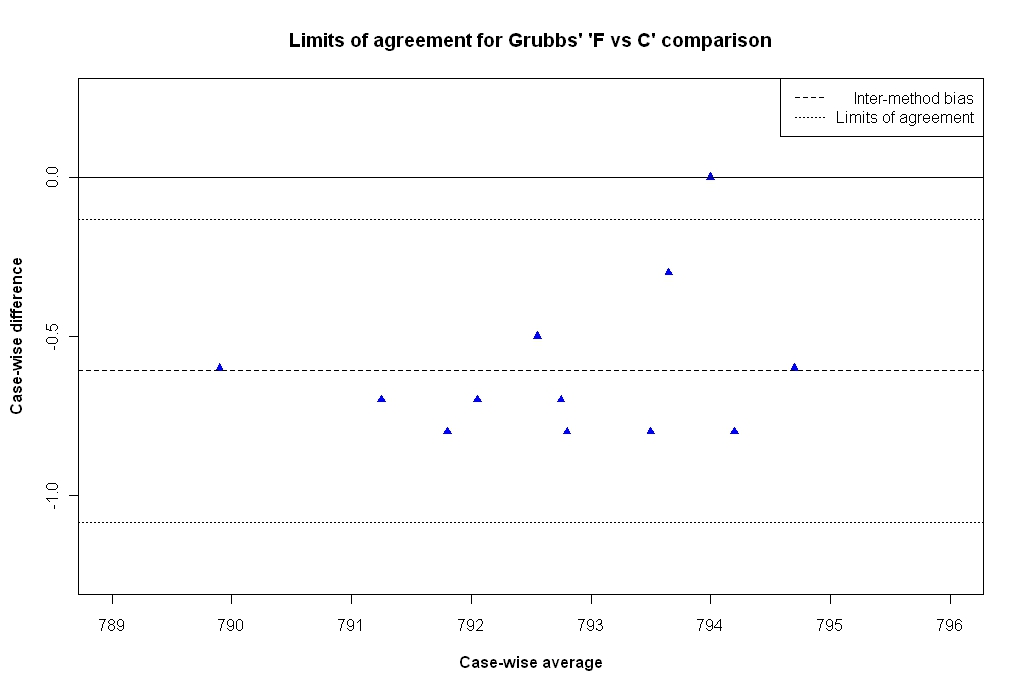
\includegraphics[width=125mm]{GrubbsBAplot-LOA.jpeg}
	%		\caption{Bland-Altman plot with limits of agreement}\label{GrubbsBAplot-noLOA}
	%	\end{center}
	%\end{figure}
	
	The limits of agreement methodology assumes a constant level of
	bias throughout the range of measurements. As \citet*{BA86} point
	out this may not be the case. Bland and Altman advises on how to
	calculate of confidence intervals for the inter-method bias and
	the limits of agreement. Importantly the authors recommend prior
	determination of what would and would constitute acceptable
	agreement, and that sample sizes should be predetermined to give
	an accurate conclusion.
	
	\begin{quote}
		`How far apart measurements can be without causing difficulties
		will be a question of judgment. Ideally, it should be defined in
		advance to help in the interpretation of the method comparison and
		to choose the sample size.'\citep{BA86}
	\end{quote}
	
	%\subsubsection{Small Sample Sizes} The limits of agreement are
	%estimates derived from the sample studied, and will differ from
	%values relevant to the whole population, hence the importance of a
	%suitably large sample size. A different sample would give
	%different limits of agreement. Student's t-distribution is a well
	%known probability distribution used in statistical inference for
	%normally distributed populations when the sample size is small
	%\citep{student,Fisher3}. Consequently, using 't' quantiles , as
	%opposed to standard normal quantiles, may give a more appropriate
	%calculation for limits of agreement when the sample size is small.
	%For sample size $n=12$ the `t' quantile is 2.2 and the limits of
	%agreement are (-0.074,-1.143).
	\citet{BA99} note the similarity of limits of agreement to
	confidence intervals, but are clear that they are not the same
	thing. Interestingly, they describe the limits as ``being like a
	reference interval."
	
	Limits of agreement have very similar construction to Shewhart
	control limits. The Shewhart chart is a well known graphical
	methodology used in statistical process control. Consequently
	there is potential for misinterpreting the limits of agreement as
	if equivalent to Shewhart control limits. Importantly the
	parameters used to determine the limits, the mean and standard
	deviation, are not based on any sample used for an analysis, but
	on the process's historical values, a key difference with
	Bland-Altman limits of agreement.
	
	\citet{BXC2008} regards the limits of agreement as a prediction
	interval for the difference between future measurements with the
	two methods on a new individual, but states that it does not fit
	the formal definition of a prediction interval, since the
	definition does not consider the errors in estimation of the
	parameters. Prediction intervals, which are often used in
	regression analysis, are estimates of an interval in which future
	observations will fall, with a certain probability, given what has
	already been observed. \citet{BXC2008} offers an alternative
	formulation, a $95\%$ prediction interval for the difference
	\begin{equation}
	\bar{d} \pm t_{(0.975, n-1)}S_{d} \sqrt{1+\frac{1}{n}}
	\end{equation}
	
	\noindent where $n$ is the number of subjects. Only for 61 or more
	subjects is there a quantile less than 2.
	
	\citet{luiz} describes limits of agreement as tolerance limits. A
	tolerance interval for a measured quantity is the interval in
	which a specified fraction of the population's values lie, with a
	specified level of confidence.
	
	%At least 100 historical
	%values must be used to determine the acceptable value (i.e the
	%process mean) and the process standard deviation. The principle
	%that the mean and variance of a large sample of a homogeneous
	%population is a close approximation of the population's mean and
	%variance justifies this.
	

	\subsection{Problems with Limits of Agreement}
	
	Several problems have been highlighted regarding Limits of
	Agreement. One is the somewhat arbitrary manner in which they are
	constructed. While in essence a confidence interval, they are not
	constructed a such. They are designed for future values.
	\\
	The formulation is also heavily influenced by outliers. An Example
	in \citet*{BA83} demonstrates the effect of recalculating without
	a particular outlier. Refering to the VCF data set in the same
	paper, there is more than one outlier.
	
	

	\section{The Bland Altman Plot}
	In 1986 Bland and Altman published a paper in the Lancet proposing
	the difference plot for use for method comparison purposes. It has
	proved highly popular ever since. This is a simple, and widely
	used , plot of the differences of each data pair, and the
	corresponding average value. An important requirement is that the
	two measurement methods use the same scale of measurement.
	\\
	Variations of the Bland Altman plot is the use of ratios, in the
	place of differences.
	\begin{equation}
	D_{i} = X_{i} - Y_{i}   \label{BA01}
	\end{equation}
	Altman and Bland suggest plotting the within subject differences $
	D = X_{1} - X_{2} $ on the ordinate versus the average of $x_{1}$
	and  $x_{2}$ on the abscissa.
	

	
	
	\section{Bland-Altman Plots}
	The issue of whether two measurement methods comparable to the
	extent that they can be used interchangeably with sufficient
	accuracy is encountered frequently in scientific research.
	Historically comparison of two methods of measurement was carried
	out by use of paired sample t-test, correlation coefficients or
	simple linear regression. Statisticians Martin Bland and Douglas
	Altman recognized the inadequacies of these analyses and
	articulated quite thoroughly the basis on which of which they are
	unsuitable for comparing two methods of measurement \citep*{BA83}.
	Furthermore they proposed their simple methodology specifically
	constructed for method comparison studies. They acknowledge the
	opportunity to apply other valid, but complex, methodologies, but
	argue that a simple approach is preferable, especially when the
	results must be `explained to non-statisticians'.
	
	Notwithstanding previous remarks about regression, the first step
	recommended, which the authors argue should be mandatory, is
	construction of a simple scatter plot of the data. The line of
	equality should also be shown, as it is necessary to give the
	correct interpretation of how both methods compare. A scatter plot
	of the Grubbs data is shown in Figure 1.1. Visual inspection confirms the previous conclusion that there is an
	inter-method bias present, i.e. Fotobalk device has a tendency to
	record a lower velocity.
	
	\begin{figure}[h!]
		\begin{center}
			\includegraphics[width=130mm]{images/GrubbsScatter.jpeg}
			\caption{Scatter plot For Fotobalk and Counter Methods.}\label{GrubbsScatter}
		\end{center}
	\end{figure}
	
	In light of shortcomings associated with scatterplots,
	\citet*{BA83} recommend a further analysis of the data. Firstly
	case-wise differences of measurements of two methods $d_{i} =
	y_{1i}-y_{2i} \mbox{ for }i=1,2,..n$ on the same subject should be
	calculated, and then the average of those measurements ($a_{i} =
	(y_{1i} + y_{2i})/2 \mbox{ for }i=1,2,..n$). These differences and
	averages are then plotted. This methodology, now commonly known as
	the `Bland-Altman Plot', has proved very successful.
	\citet*{BA86}, which further develops the methodology, was found
	to be the sixth most cited paper of all time by the
	\citet{BAcite}. \cite{Dewitte} also commented on the rate at which
	prevalence of the Bland-Altman plot has developed in scientific
	literature. The Bland-Altman Plot has since become expected, and
	often obligatory, approach for presenting method comparison
	studies in many scientific journals \citep{hollis}. Furthermore
	\citet{BritHypSoc} recommend its use in papers pertaining to
	method comparison studies for the journal of the British
	Hypertension Society.
	
	The magnitude of the inter-method bias between the two methods is
	simply the average of the differences $\bar{d}$. The variances
	around this bias is estimated by the standard deviation of the
	differences $S(d)$. This inter-method bias is represented with a
	line on the Bland-Altman plot. These estimates are only meaningful
	if there is uniform inter-bias and variability throughout the
	range of measurements, which can be checked by visual inspection
	of the plot. In the case of Grubbs data the inter-method bias is
	$-0.61$ metres per second, and is indicated by the dashed line on
	Figure 1.2. By inspection of the plot, it is also possible to
	compare the precision of each method. Noticeably the differences
	tend to increase as the averages increase.
	
	
	\begin{table}[h!]
		\renewcommand\arraystretch{0.7}%
		\begin{center}
			\begin{tabular}{|c||c|c||c|c|}
				\hline
				Round & Fotobalk  & Counter  & Differences  & Averages  \\
				&  [F] & [C] & [F-C] &  [(F+C)/2] \\
				\hline
				1 & 793.8 & 794.6 & -0.8 & 794.2 \\
				2 & 793.1 & 793.9 & -0.8 & 793.5 \\
				3 & 792.4 & 793.2 & -0.8 & 792.8 \\
				4 & 794.0 & 794.0 & 0.0 & 794.0 \\
				5 & 791.4 & 792.2 & -0.8 & 791.8 \\
				6 & 792.4 & 793.1 & -0.7 & 792.8 \\
				7 & 791.7 & 792.4 & -0.7 & 792.0 \\
				8 & 792.3 & 792.8 & -0.5 & 792.5 \\
				9 & 789.6 & 790.2 & -0.6 & 789.9 \\
				10 & 794.4 & 795.0 & -0.6 & 794.7 \\
				11 & 790.9 & 791.6 & -0.7 & 791.2 \\
				12 & 793.5 & 793.8 & -0.3 & 793.6 \\
				\hline
			\end{tabular}
			\caption{Fotobalk and Counter methods: differences and averages.}
		\end{center}
	\end{table}
	
	\begin{table}[h!]
		\renewcommand\arraystretch{0.7}%
		\begin{center}
			\begin{tabular}{|c||c|c||c|c|}
				\hline
				Round & Fotobalk  & Terma  & Differences  & Averages  \\
				&  [F] & [T] & [F-T] &  [(F+T)/2] \\
				\hline
				1 & 793.80 & 793.20 & 0.60 & 793.50 \\
				2 & 793.10 & 793.30 & -0.20 & 793.20 \\
				3 & 792.40 & 792.60 & -0.20 & 792.50 \\
				4 & 794.00 & 793.80 & 0.20 & 793.90 \\
				5 & 791.40 & 791.60 & -0.20 & 791.50 \\
				6 & 792.40 & 791.60 & 0.80 & 792.00 \\
				7 & 791.70 & 791.60 & 0.10 & 791.65 \\
				8 & 792.30 & 792.40 & -0.10 & 792.35 \\
				9 & 789.60 & 788.50 & 1.10 & 789.05 \\
				10 & 794.40 & 794.70 & -0.30 & 794.55 \\
				11 & 790.90 & 791.30 & -0.40 & 791.10 \\
				12 & 793.50 & 793.50 & 0.00 & 793.50 \\
				
				\hline
			\end{tabular}
			\caption{Fotobalk and Terma methods: differences and averages.}
		\end{center}
	\end{table}
	
	\newpage
	
	
	\subsection{Using Bland-Altman Plots}
	Bland-Altman plots are a powerful graphical methodology for making
	a visual assessment of the data. \citet*{BA83} express the
	motivation for this plot thusly:
	\begin{quote}
		``From this type of plot it is much easier to assess the magnitude
		of disagreement (both error and bias), spot outliers, and see
		whether there is any trend, for example an increase in
		(difference) for high values. This way of plotting the data is a
		very powerful way of displaying the results of a method comparison
		study."
	\end{quote}
	
	The Bland-Altman plot is simply a scatterplot of the case-wise
	averages and differences of two methods of measurement. As the
	objective of the Bland-Altman plot is to advise on the agreement
	of two methods, it is the case-wise differences that are
	particularly. Later it will be shown that case-wise differences
	are the sole component of the next part of the methodology, the
	limits of agreement.
	
	For creating plots, the case wise-averages fulfil several
	functions, such as expressing the range over which the values were
	taken, and assessing whether the assumptions of constant variance
	holds. Case-wise averages also allow the case-wise differences to
	be presented on a two-dimensional plot, with better data
	visualization qualities than a one dimensional plot. \citet{BA86}
	cautions that it would be the difference against either
	measurement value instead of their average , as the difference
	relates to both value.
	
	The Bland-Altman plot for comparing the `Fotobalk' and `Counter'
	methods, which shall henceforth be referred to as the `F vs C'
	comparison,  is depicted in Figure 1.2, using data from Table 1.3.
	The presence and magnitude of the inter-method bias is indicated
	by the dashed line.
	
	\begin{figure}[h!]
		\begin{center}
			\includegraphics[width=120mm]{images/GrubbsBAplot-noLOA.jpeg}
			\caption{Bland-Altman plot For Fotobalk and Counter methods.}\label{GrubbsBA-noLOA}
		\end{center}
	\end{figure}
	
	
	
	In Figure 1.3 Bland-Altman plots for the `F vs C' and `F vs T'
	comparisons are shown, where `F vs T' refers to the comparison of
	the `Fotobalk' and `Terma' methods. Usage of the Bland-Altman plot
	can be demonstrate in the contrast between these comparisons.
	
	\begin{figure}[h!]
		\begin{center}
			\includegraphics[height=90mm]{images/GrubbsDataTwoBAplots.jpeg}
			\caption{Bland-Altman plots for Grubbs' F vs C and F vs T comparisons.}\label{GrubbsDataTwoBAplots}
		\end{center}
	\end{figure}
	
	By inspection, there exists a larger inter-method bias in the `F
	vs C' comparison than in the `F vs T' comparison. Conversely there
	appears to be less precision in`F vs T' comparison, as indicated
	by the greater dispersion of co-variates.
	
	Figures 1.4, 1.5 and 1.6 are three prototype Bland-Altman plots
	derived from simulated data, each for the purpose of demonstrating
	how the plot would inform an analyst of features that would
	adversely affect use of the recommended methodology.
	
	Figure 1.4 demonstrates how the Bland-Altman plot would indicate
	increasing variance of differences over the measurement range.
	Fitted regression lines, for both the upper and lower half of the
	plot, has been added to indicate the trend. Figure 1.5 is an
	example of cases where the inter-method bias changes over the
	measurement range. This is known as proportional bias. In both
	Figures 1.4 and 1.5, the assumptions necessary for further
	analysis using the limits of agreement are violated.
	
	Application of regression techniques to the Bland-Altman plot, and
	subsequent formal testing for the constant variability of
	differences is informative. The data set may be divided into two
	subsets, containing the observations wherein the difference values
	are less than and greater than the inter-method bias respectively.
	For both of these fits, hypothesis tests for the respective slopes
	can be performed. While both tests can be considered separately,
	multiple comparison procedures, such as the Benjamini-Hochberg
	\citep{BH} test, should be also be used.
	
	\begin{figure}[h!]
		\begin{center}
			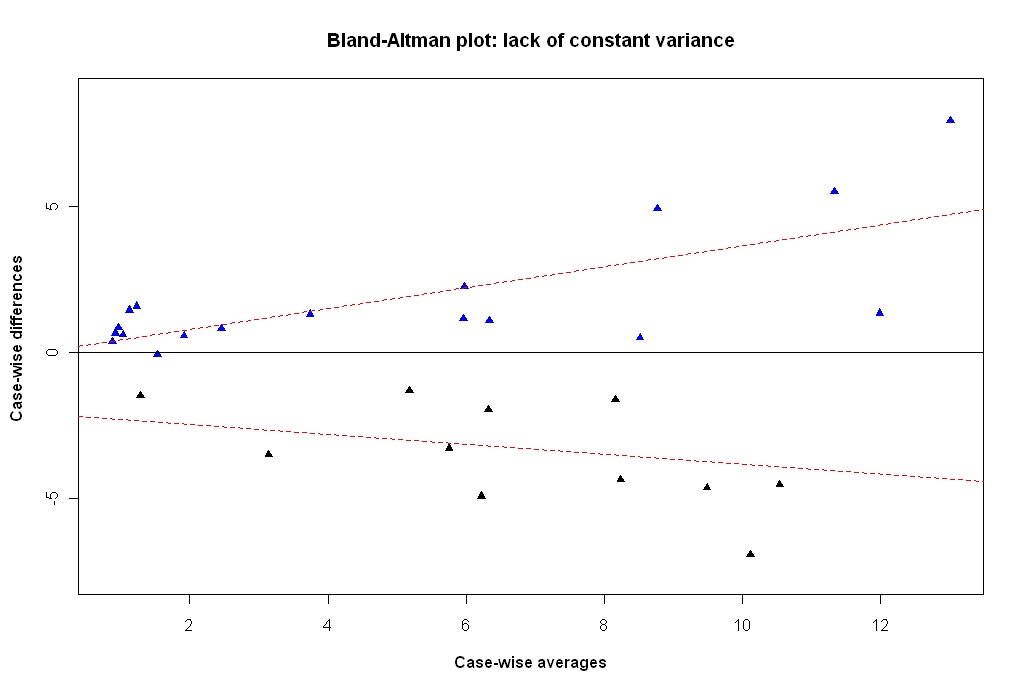
\includegraphics[height=90mm]{images/BAFanEffect.jpeg}
			\caption{Bland-Altman plot demonstrating the increase of variance over the range.}\label{BAFanEffect}
		\end{center}
	\end{figure}
	
	\begin{figure}[h!]
		\begin{center}
			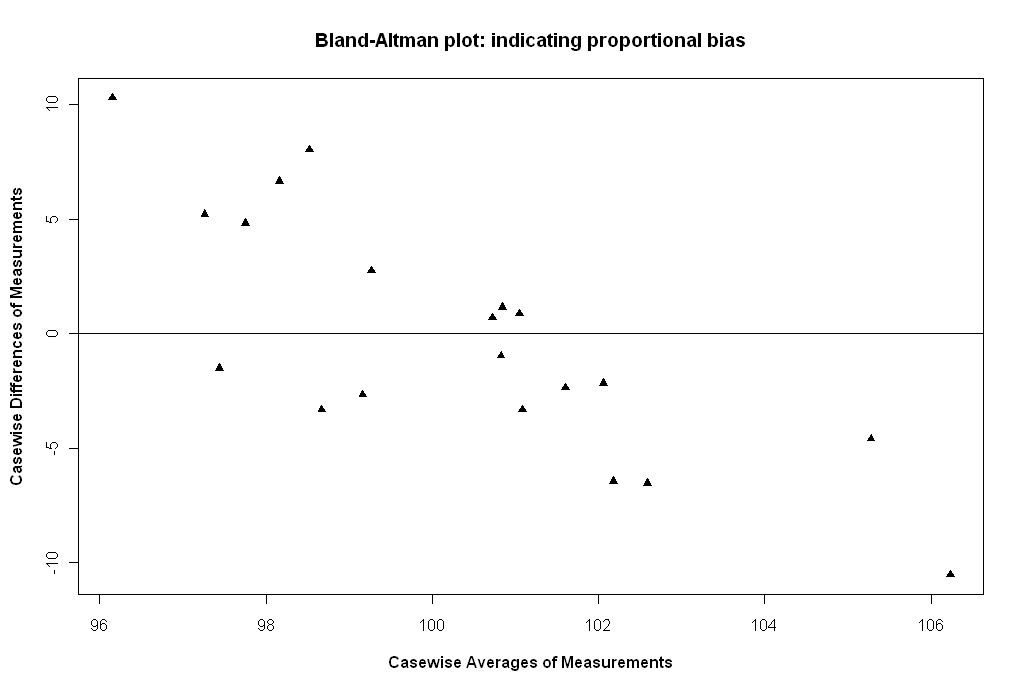
\includegraphics[height=90mm]{images/PropBias.jpeg}
			\caption{Bland-Altman plot indicating the presence of proportional bias.}\label{PropBias}
		\end{center}
	\end{figure}
	
	\begin{figure}[h!]
		\begin{center}
			\includegraphics[width=125mm]{images/BAOutliers.jpeg}
			\caption{Bland-Altman plot indicating the presence of potential outliers.}\label{Outliers}
		\end{center}
	\end{figure}
	
	
	% outliers
	
	
	The Bland-Altman plot also can be used to identify outliers. An
	outlier is an observation that is conspicuously different from the
	rest of the data that it arouses suspicion that it occurs due to a
	mechanism, or conditions, different to that of the rest of the
	observations. Classification of outliers can be determined with
	numerous established approaches, such as the Grubb's test, but
	always classification must be informed by the logic of the data's
	formulation. Figure 1.6 is a Bland-Altman plot with two potential
	outliers.
	
	
	\citet*{BA99} do not recommend excluding outliers from analyses,
	but remark that recalculation of the inter-method bias estimate,
	and further calculations based upon that estimate, are useful for
	assessing the influence of outliers. The authors remark that `we
	usually find that this method of analysis is not too sensitive to
	one or two large outlying differences'.
	
	
	%\citet{Grubbs} defined an outlier as a co-variate that appears to
	%deviate markedly from other members of the sample in which it
	%occurs.
	
	In classifying whether a observation from a univariate data set is
	an outlier, Grubbs' outlier test is widely used. In assessing
	whether a co-variate in a Bland-Altman plot is an outlier, this
	test is useful when applied to the difference values treated as a
	univariate data set. For Grubbs' data, this outlier test is
	carried out on the differences, yielding the following results.
	
	The null and alternative hypotheses is the absence and presence of
	at least one outlier respectively. Grubbs' outlier test statistic
	$G$ is the largest absolute deviation from the sample mean divided
	by the standard deviation of the differences. For the `F vs C'
	comparison, $G = 3.6403$. The critical value is calculated using
	Student's $t$ distribution and the sample size,
	\begin{equation}
	U = \frac{n-1}{\sqrt{n}} \sqrt{\frac{t_{\alpha/(2n),n-2}^2}{n - 2
			+ t_{\alpha/(2n),n-2}^2}}.
	\end{equation}
	
	For this test $U = 0.7501$. The conclusion of this test is that
	the fourth observation in the `F vs C' comparison is an outlier,
	with $p-value = 0.002799$.
	
	As a complement to the Bland-Altman plot, \citet{Bartko} proposes
	the use of a bivariate confidence ellipse, constructed for a
	predetermined level.
	
	The minor axis relates to the between subject variability, whereas
	the major axis relates to the error mean square, with the ellipse
	depicting the size of both relative to each
	other.\citet{AltmanEllipse} provides the relevant calculations for
	the ellipse. Bartko states that the ellipse can, inter alia, be
	used to detect the presence of outliers (furthermore
	\citet{Bartko} proposes formal testing procedures, that shall be
	discussed in due course). Inspection of Figure 1.7 shows that the
	fourth observation is outside the bounds of the ellipse,
	concurring with the conclusion that it is an outlier.
	
	
	\begin{figure}[h!]
		% Requires \usepackage{graphicx}
		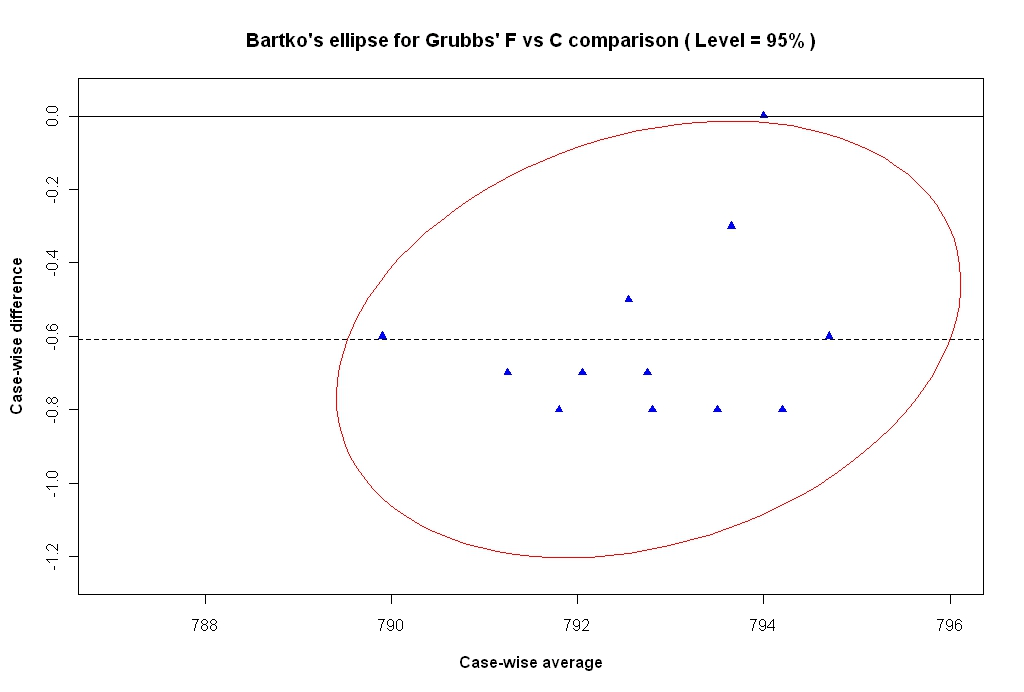
\includegraphics[width=130mm]{images/GrubbsBartko.jpeg}
		\caption{Bartko's Ellipse For Grubbs' Data.}\label{GrubbsBartko}
	\end{figure}
	
	The limitations of using bivariate approaches to outlier detection
	in the Bland-Altman plot can demonstrated using Bartko's ellipse.
	A co-variate is added to the `F vs C' comparison that has a
	difference value equal to the inter-method bias, and an average
	value that markedly deviates from the rest of the average values
	in the comparison, i.e. 786. Table 1.8 depicts a $95\%$ confidence
	ellipse for this enhanced data set. By inspection of the
	confidence interval, a conclusion would be reached that this extra
	co-variate is an outlier, in spite of the fact that this
	observation is consistent with the intended conclusion of the
	Bland-Altman plot.
	
	\begin{figure}[h!]
		% Requires \usepackage{graphicx}
		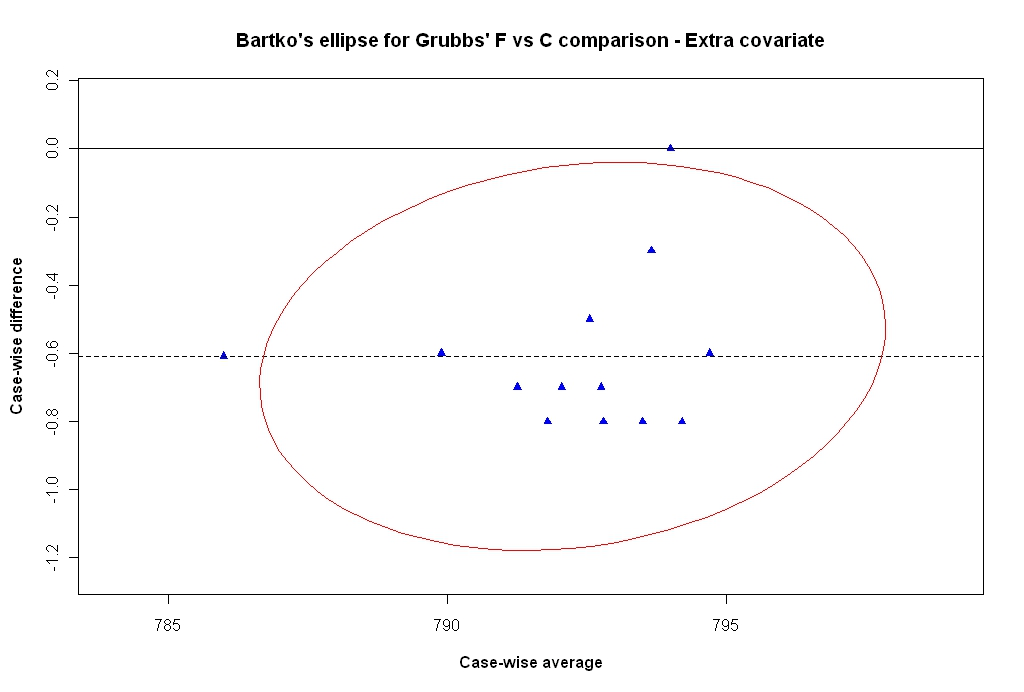
\includegraphics[width=130mm]{images/GrubbsBartko2.jpeg}
		\caption{Bartko's Ellipse For Grubbs' Data, with an extra covariate.}\label{GrubbsBartko2}
	\end{figure}
	
	In the Bland-Altman plot, the horizontal displacement of any
	observation is supported by two independent measurements. Any
	observation should not be considered an outlier on the basis of a
	noticeable horizontal displacement from the main cluster, as in
	the case with the extra co-variate. Conversely, the fourth
	observation, from the original data set, should be considered an
	outlier, as it has a noticeable vertical displacement from the
	rest of the observations.
	
	Bartko's ellipse provides a visual aid to determining the
	relationship between variances. If $\mbox{var}(a_{i})$ is greater
	than $\mbox{var}(d_{i})$, the orientation of the ellipse is
	horizontal. Conversely if $\mbox{var}(a_{i})$ is less than
	$\mbox{var}(d_{i})$, the orientation of the ellipse is vertical.
	\newpage
	
	
	
	%\begin{figure}[h!]
	%\begin{center}
	%  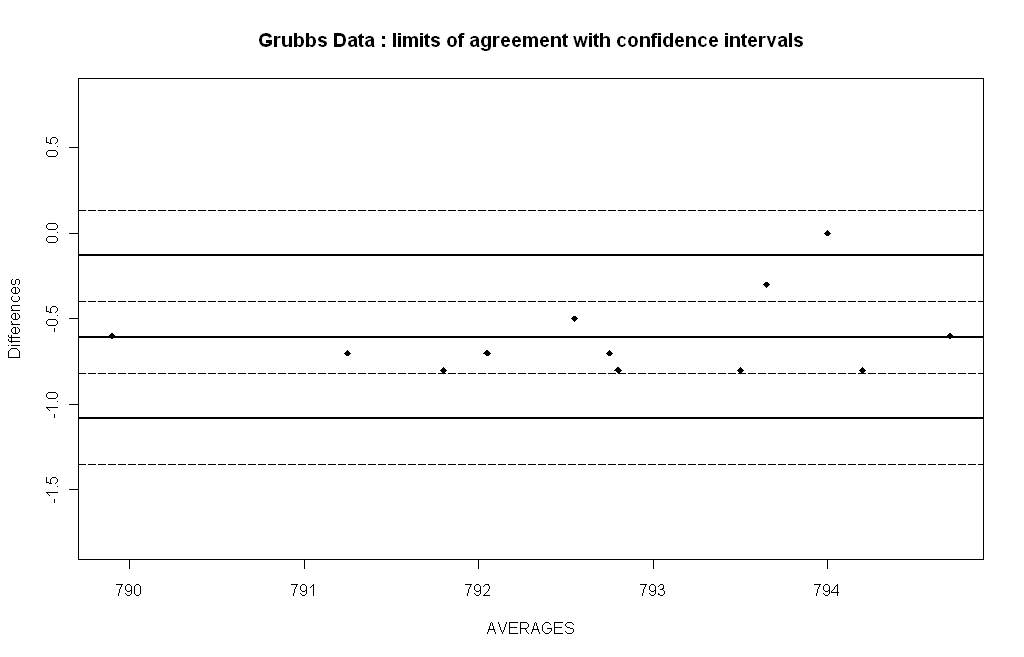
\includegraphics[width=125mm]{images/GrubbsLOAwCIs.jpeg}
	%  \caption{Limits of agreement with confidence intervals}\label{LOAwCIs}
	%\end{center}
	%\end{figure}
	
	\subsection{Using Bland-Altman Plots}
	Bland-Altman plots are a powerful graphical methodology for making
	a visual assessment of the data. \citet*{BA83} express the
	motivation for this plot thusly:
	\begin{quote}
		``From this type of plot it is much easier to assess the magnitude
		of disagreement (both error and bias), spot outliers, and see
		whether there is any trend, for example an increase in
		(difference) for high values. This way of plotting the data is a
		very powerful way of displaying the results of a method comparison
		study."
	\end{quote}
	
	The Bland-Altman plot is simply a scatterplot of the case-wise
	averages and differences of two methods of measurement. As the
	objective of the Bland-Altman plot is to advise on the agreement
	of two methods, it is the case-wise differences that are
	particularly. Later it will be shown that case-wise differences
	are the sole component of the next part of the methodology, the
	limits of agreement.
	
	For creating plots, the case wise-averages fulfil several
	functions, such as expressing the range over which the values were
	taken, and assessing whether the assumptions of constant variance
	holds. Case-wise averages also allow the case-wise differences to
	be presented on a two-dimensional plot, with better data
	visualization qualities than a one dimensional plot. \citet{BA86}
	cautions that it would be the difference against either
	measurement value instead of their average , as the difference
	relates to both value.
	
	The Bland-Altman plot for comparing the `Fotobalk' and `Counter'
	methods, which shall henceforth be referred to as the `F vs C'
	comparison,  is depicted in Figure 1.2, using data from Table 1.3.
	The presence and magnitude of the inter-method bias is indicated
	by the dashed line.
	
	\begin{figure}[h!]
		\begin{center}
			\includegraphics[width=120mm]{images/GrubbsBAplot-noLOA.jpeg}
			\caption{Bland-Altman plot For Fotobalk and Counter methods.}\label{GrubbsBA-noLOA}
		\end{center}
	\end{figure}
	
	
	
	In Figure 1.3 Bland-Altman plots for the `F vs C' and `F vs T'
	comparisons are shown, where `F vs T' refers to the comparison of
	the `Fotobalk' and `Terma' methods. Usage of the Bland-Altman plot
	can be demonstrate in the contrast between these comparisons.
	
	\begin{figure}[h!]
		\begin{center}
			\includegraphics[height=90mm]{images/GrubbsDataTwoBAplots.jpeg}
			\caption{Bland-Altman plots for Grubbs' F vs C and F vs T comparisons.}\label{GrubbsDataTwoBAplots}
		\end{center}
	\end{figure}
	
	By inspection, there exists a larger inter-method bias in the `F
	vs C' comparison than in the `F vs T' comparison. Conversely there
	appears to be less precision in`F vs T' comparison, as indicated
	by the greater dispersion of co-variates.
	
	Figures 1.4, 1.5 and 1.6 are three prototype Bland-Altman plots
	derived from simulated data, each for the purpose of demonstrating
	how the plot would inform an analyst of features that would
	adversely affect use of the recommended methodology.
	
	Figure 1.4 demonstrates how the Bland-Altman plot would indicate
	increasing variance of differences over the measurement range.
	Fitted regression lines, for both the upper and lower half of the
	plot, has been added to indicate the trend. Figure 1.5 is an
	example of cases where the inter-method bias changes over the
	measurement range. This is known as proportional bias. In both
	Figures 1.4 and 1.5, the assumptions necessary for further
	analysis using the limits of agreement are violated.
	
	Application of regression techniques to the Bland-Altman plot, and
	subsequent formal testing for the constant variability of
	differences is informative. The data set may be divided into two
	subsets, containing the observations wherein the difference values
	are less than and greater than the inter-method bias respectively.
	For both of these fits, hypothesis tests for the respective slopes
	can be performed. While both tests can be considered separately,
	multiple comparison procedures, such as the Benjamini-Hochberg
	\citep{BH} test, should be also be used.
	
	\begin{figure}[h!]
		\begin{center}
			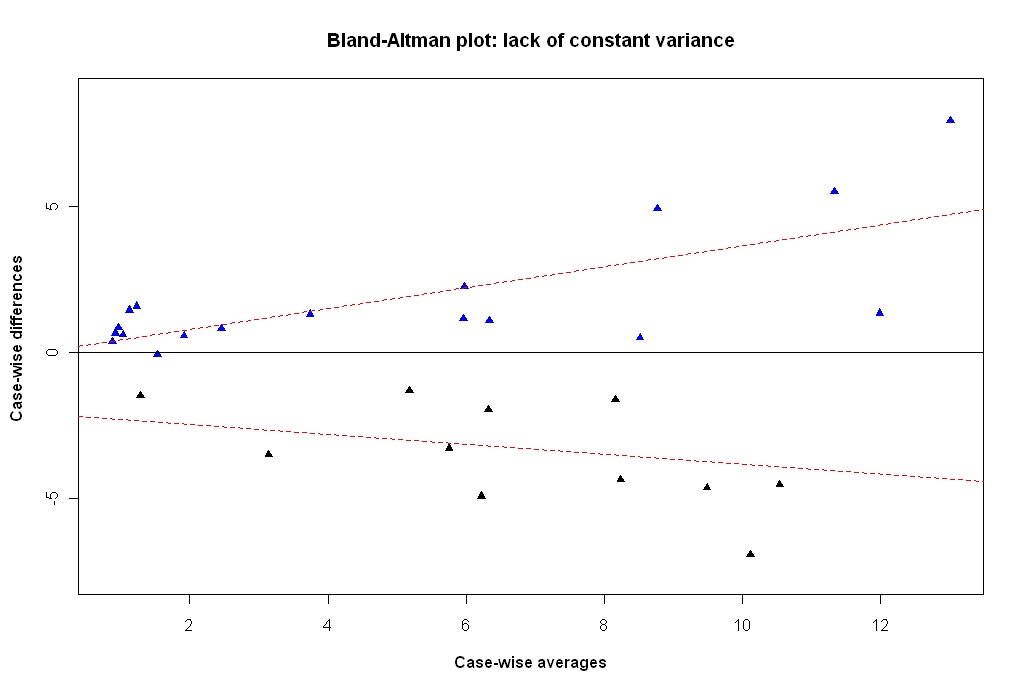
\includegraphics[height=90mm]{images/BAFanEffect.jpeg}
			\caption{Bland-Altman plot demonstrating the increase of variance over the range.}\label{BAFanEffect}
		\end{center}
	\end{figure}
	
	\begin{figure}[h!]
		\begin{center}
			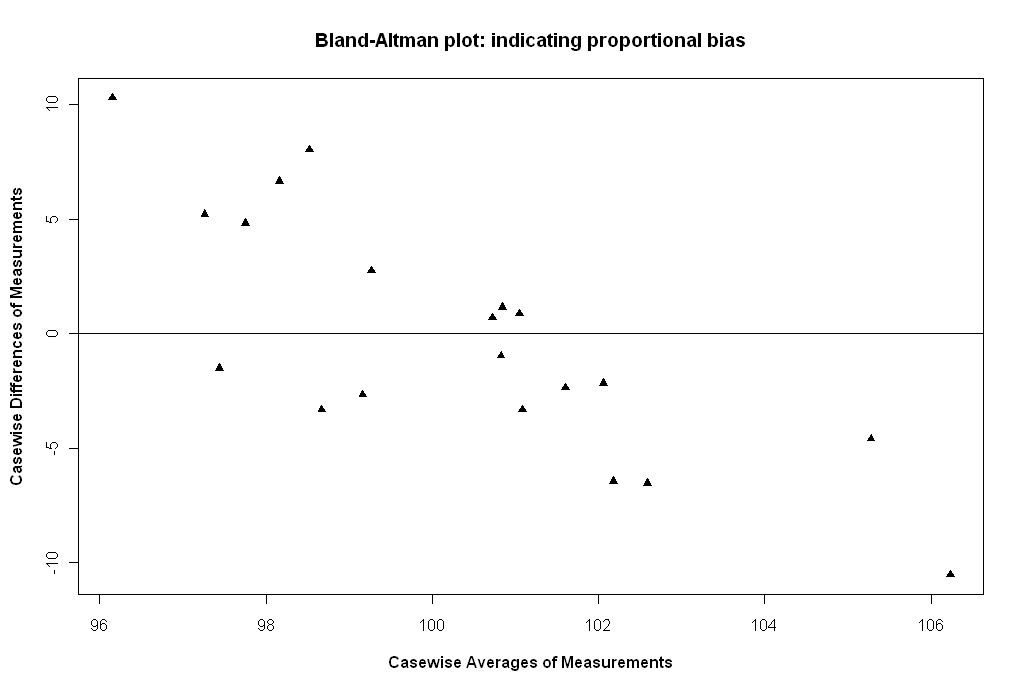
\includegraphics[height=90mm]{images/PropBias.jpeg}
			\caption{Bland-Altman plot indicating the presence of proportional bias.}\label{PropBias}
		\end{center}
	\end{figure}
	
	\begin{figure}[h!]
		\begin{center}
			\includegraphics[width=125mm]{images/BAOutliers.jpeg}
			\caption{Bland-Altman plot indicating the presence of potential outliers.}\label{Outliers}
		\end{center}
	\end{figure}
	
	
	% outliers
	
	
	The Bland-Altman plot also can be used to identify outliers. An
	outlier is an observation that is conspicuously different from the
	rest of the data that it arouses suspicion that it occurs due to a
	mechanism, or conditions, different to that of the rest of the
	observations. Classification of outliers can be determined with
	numerous established approaches, such as the Grubb's test, but
	always classification must be informed by the logic of the data's
	formulation. Figure 1.6 is a Bland-Altman plot with two potential
	outliers.
	
	
	\citet*{BA99} do not recommend excluding outliers from analyses,
	but remark that recalculation of the inter-method bias estimate,
	and further calculations based upon that estimate, are useful for
	assessing the influence of outliers. The authors remark that `we
	usually find that this method of analysis is not too sensitive to
	one or two large outlying differences'.
	
	
	%\citet{Grubbs} defined an outlier as a co-variate that appears to
	%deviate markedly from other members of the sample in which it
	%occurs.
	
	In classifying whether a observation from a univariate data set is
	an outlier, Grubbs' outlier test is widely used. In assessing
	whether a co-variate in a Bland-Altman plot is an outlier, this
	test is useful when applied to the difference values treated as a
	univariate data set. For Grubbs' data, this outlier test is
	carried out on the differences, yielding the following results.
	
	The null and alternative hypotheses is the absence and presence of
	at least one outlier respectively. Grubbs' outlier test statistic
	$G$ is the largest absolute deviation from the sample mean divided
	by the standard deviation of the differences. For the `F vs C'
	comparison, $G = 3.6403$. The critical value is calculated using
	Student's $t$ distribution and the sample size,
	\begin{equation}
	U = \frac{n-1}{\sqrt{n}} \sqrt{\frac{t_{\alpha/(2n),n-2}^2}{n - 2
			+ t_{\alpha/(2n),n-2}^2}}.
	\end{equation}
	
	For this test $U = 0.7501$. The conclusion of this test is that
	the fourth observation in the `F vs C' comparison is an outlier,
	with $p-value = 0.002799$.
	
	As a complement to the Bland-Altman plot, \citet{Bartko} proposes
	the use of a bivariate confidence ellipse, constructed for a
	predetermined level.
	
	The minor axis relates to the between subject variability, whereas the major axis relates to the error mean square, with the ellipse
	depicting the size of both relative to each	other.\citet{AltmanEllipse} provides the relevant calculations for
	the ellipse. Bartko states that the ellipse can, inter alia, be
	used to detect the presence of outliers (furthermore \citet{Bartko} proposes formal testing procedures, that shall be
	discussed in due course). Inspection of Figure 1.7 shows that the
	fourth observation is outside the bounds of the ellipse, concurring with the conclusion that it is an outlier.
	
	
	\begin{figure}[h!]
		% Requires \usepackage{graphicx}
		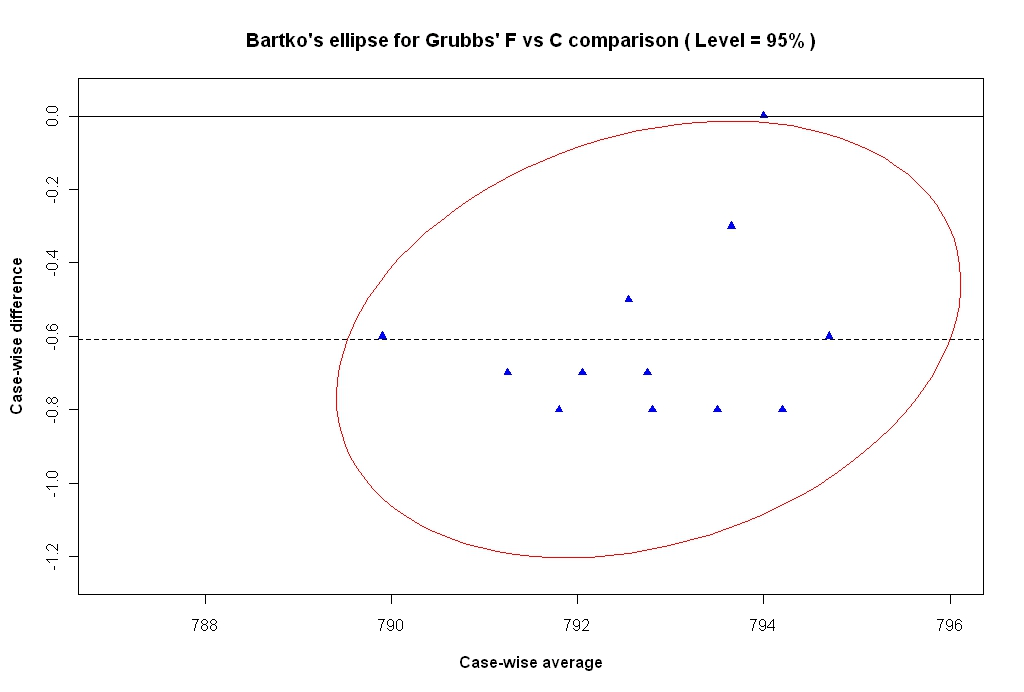
\includegraphics[width=130mm]{images/GrubbsBartko.jpeg}
		\caption{Bartko's Ellipse For Grubbs' Data.}\label{GrubbsBartko}
	\end{figure}
	
	The limitations of using bivariate approaches to outlier detection
	in the Bland-Altman plot can demonstrated using Bartko's ellipse.
	A co-variate is added to the `F vs C' comparison that has a	difference value equal to the inter-method bias, and an average	value that markedly deviates from the rest of the average values in the comparison, i.e. 786. Table 1.8 depicts a $95\%$ confidence
	ellipse for this enhanced data set. By inspection of the confidence interval, a conclusion would be reached that this extra
	co-variate is an outlier, in spite of the fact that this observation is consistent with the intended conclusion of the
	Bland-Altman plot.
	
	\begin{figure}[h!]
		% Requires \usepackage{graphicx}
		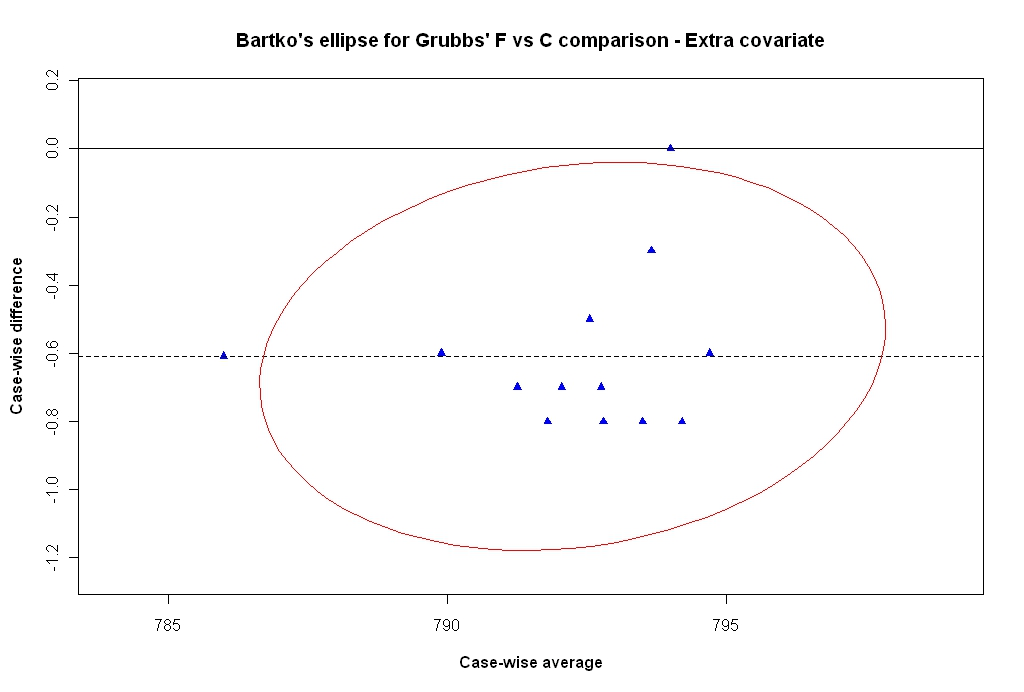
\includegraphics[width=130mm]{images/GrubbsBartko2.jpeg}
		\caption{Bartko's Ellipse For Grubbs' Data, with an extra covariate.}\label{GrubbsBartko2}
	\end{figure}
	
	In the Bland-Altman plot, the horizontal displacement of any observation is supported by two independent measurements. Any
	observation should not be considered an outlier on the basis of a
	noticeable horizontal displacement from the main cluster, as in
	the case with the extra co-variate. Conversely, the fourth observation, from the original data set, should be considered an
	outlier, as it has a noticeable vertical displacement from the rest of the observations.
	
	Bartko's ellipse provides a visual aid to determining the relationship between variances. If $\mbox{var}(a_{i})$ is greater
	than $\mbox{var}(d_{i})$, the orientation of the ellipse is	horizontal. Conversely if $\mbox{var}(a_{i})$ is less than
	$\mbox{var}(d_{i})$, the orientation of the ellipse is vertical.
	\newpage
	
	
	
	%\begin{figure}[h!]
	%\begin{center}
	%  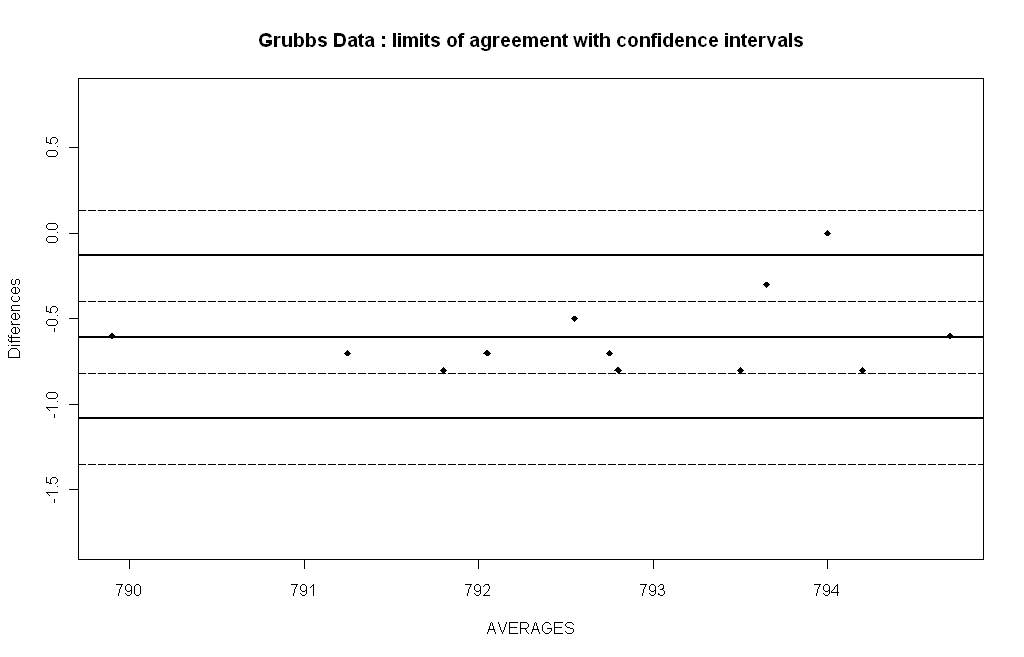
\includegraphics[width=125mm]{images/GrubbsLOAwCIs.jpeg}
	%  \caption{Limits of agreement with confidence intervals}\label{LOAwCIs}
	%\end{center}
	%\end{figure}
	
	%================================================================ %
	% USED

	\subsection{Regression-based Limits of Agreement} Assuming that
	there will be no curvature in the scatter-plot, the methodology
	regresses the difference of methods ($d$) on the average of those
	methods ($a$) with a simple intercept slope model; $\hat{d} =
	b_{0}+ b_{1}a.$ Should the slope $b_{1}$ be found to be
	negligible, $\hat{d}$ takes the value $\bar{d}$.
	
	The next step to take in calculating the limits is also a
	regression, this time of the residuals as a function of the scale
	of the measurements, expressed by the averages $a_{i}$;
	$ \hat{R} = c_{0}+ c_{1}a_{i}$
	
	With reference to absolute values following a half-normal
	distribution with mean $\sigma\sqrt{\frac{2}{\pi}}$, \citet{BA99} formulate the regression based limits of agreement as
	follows
	\begin{equation}
	\hat{d} \pm 1.96\sqrt{\frac{\pi}{2}}\hat{R} = \hat{d} \pm 2.46\hat{R}
	\end{equation}
	
	\subsection{Regression-based Limits of Agreement} Assuming that
	there will be no curvature in the scatter-plot, the methodology
	regresses the difference of methods ($d$) on the average of those
	methods ($a$) with a simple intercept slope model; $\hat{d} =
	b_{0}+ b_{1}a.$ Should the slope $b_{1}$ be found to be
	negligible, $\hat{d}$ takes the value $\bar{d}$.
	
	The next step to take in calculating the limits is also a
	regression, this time of the residuals as a function of the scale
	of the measurements, expressed by the averages $a_{i}$;
	$ \hat{R} = c_{0}+ c_{1}a_{i}$
	
	With reference to absolute values following a half-normal
	distribution with mean $\sigma\sqrt{\frac{2}{\pi}}$, \citet{BA99} formulate the regression based limits of agreement as
	follows
	\begin{equation}
	\hat{d} \pm 1.96\sqrt{\frac{\pi}{2}}\hat{R} = \hat{d} \pm 2.46\hat{R}
	\end{equation}





	\section{Bland Altman Plots}
	The issue of whether two measurement methods are comparable to the
	extent that they can be used interchangeably with sufficient
	accuracy is encountered frequently in scientific research.
	Historically comparison of two methods of measurement was carried
	out by use of matched pairs correlation coefficients or simple
	linear regression. Bland and Altman recognized the inadequacies of
	these analyses and articulated quite thoroughly the basis on which
	of which they are unsuitable for comparing two methods of
	measurement \citep*{BA83}.
	
	As an alternative they proposed a simple statistical methodology
	specifically appropriate for method comparison studies. They
	acknowledge that there are other valid methodologies, but argue
	that a simple approach is preferable to complex approaches,
	\emph{"especially when the results must be explained to
		non-statisticians"} \citep*{BA83}.
	
	The first step recommended which the authors argue should be
	mandatory is construction of a simple scatter plot of the data.
	The line of equality ($X=Y$) should also be shown, as it is
	necessary to give the correct interpretation of how both methods
	compare. A scatter plot of the Grubbs data is shown in figure 2.1.
	A visual inspection thereof confirms the previous conclusion that
	there is an inter method bias present, i.e. Fotobalk device has a
	tendency to record a lower velocity.
	
	
	
	In light of shortcomings associated with scatterplots,
	\citet*{BA83} recommend a further analysis of the data. Firstly
	differences of measurements of two methods on the same subject
	should  be calculated, and then the average of those measurements
	(Table 1.1). The averages of the two measurements is considered by
	Bland and Altman to the best estimate for the unknown true value.
	Importantly both methods must measure with the same units. These
	results are then plotted, with differences on the ordinate and
	averages on the abscissa (figure 1.2). \citet*{BA83}express the
	motivation for this plot thusly:
	\begin{quote}
		"From this type of plot it is much easier to assess the magnitude
		of disagreement (both error and bias), spot outliers, and see
		whether there is any trend, for example an increase in
		(difference) for high values. This way of plotting the data is a
		very powerful way of displaying the results of a method comparison
		study."
	\end{quote}
		
	\begin{figure}[h!]
		\begin{center}
			\includegraphics[width=130mm]{images/GrubbsScatter.jpeg}
			\caption{Scatter plot For Fotobalk and Counter Methods.}\label{GrubbsScatter}
		\end{center}
	\end{figure}
	
	In light of shortcomings associated with scatterplots,
	\citet*{BA83} recommend a further analysis of the data. Firstly
	case-wise differences of measurements of two methods $d_{i} =
	y_{1i}-y_{2i} \mbox{ for }i=1,2,..n$ on the same subject should be
	calculated, and then the average of those measurements ($a_{i} =
	(y_{1i} + y_{2i})/2 \mbox{ for }i=1,2,..n$). These differences and
	averages are then plotted. This methodology, now commonly known as
	the `Bland-Altman Plot', has proved very successful.
	\citet*{BA86}, which further develops the methodology, was found
	to be the sixth most cited paper of all time by the
	\citet{BAcite}. \cite{Dewitte} also commented on the rate at which
	prevalence of the Bland-Altman plot has developed in scientific
	literature. The Bland-Altman Plot has since become expected, and
	often obligatory, approach for presenting method comparison
	studies in many scientific journals \citep{hollis}. Furthermore
	\citet{BritHypSoc} recommend its use in papers pertaining to
	method comparison studies for the journal of the British
	Hypertension Society.
	
	The magnitude of the inter-method bias between the two methods is
	simply the average of the differences $\bar{d}$. The variances
	around this bias is estimated by the standard deviation of the
	differences $S(d)$. This inter-method bias is represented with a
	line on the Bland-Altman plot. These estimates are only meaningful
	if there is uniform inter-bias and variability throughout the
	range of measurements, which can be checked by visual inspection
	of the plot. In the case of Grubbs data the inter-method bias is
	$-0.61$ metres per second, and is indicated by the dashed line on
	Figure 1.2. By inspection of the plot, it is also possible to
	compare the precision of each method. Noticeably the differences
	tend to increase as the averages increase.
	
	
	\begin{table}[h!]
		\renewcommand\arraystretch{0.7}%
		\begin{center}
			\begin{tabular}{|c||c|c||c|c|}
				\hline
				Round & Fotobalk  & Counter  & Differences  & Averages  \\
				&  [F] & [C] & [F-C] &  [(F+C)/2] \\
				\hline
				1 & 793.8 & 794.6 & -0.8 & 794.2 \\
				2 & 793.1 & 793.9 & -0.8 & 793.5 \\
				3 & 792.4 & 793.2 & -0.8 & 792.8 \\
				4 & 794.0 & 794.0 & 0.0 & 794.0 \\
				5 & 791.4 & 792.2 & -0.8 & 791.8 \\
				6 & 792.4 & 793.1 & -0.7 & 792.8 \\
				7 & 791.7 & 792.4 & -0.7 & 792.0 \\
				8 & 792.3 & 792.8 & -0.5 & 792.5 \\
				9 & 789.6 & 790.2 & -0.6 & 789.9 \\
				10 & 794.4 & 795.0 & -0.6 & 794.7 \\
				11 & 790.9 & 791.6 & -0.7 & 791.2 \\
				12 & 793.5 & 793.8 & -0.3 & 793.6 \\
				\hline
			\end{tabular}
			\caption{Fotobalk and Counter methods: differences and averages.}
		\end{center}
	\end{table}
	
	\begin{table}[h!]
		\renewcommand\arraystretch{0.7}%
		\begin{center}
			\begin{tabular}{|c||c|c||c|c|}
				\hline
				Round & Fotobalk  & Terma  & Differences  & Averages  \\
				&  [F] & [T] & [F-T] &  [(F+T)/2] \\
				\hline
				1 & 793.80 & 793.20 & 0.60 & 793.50 \\
				2 & 793.10 & 793.30 & -0.20 & 793.20 \\
				3 & 792.40 & 792.60 & -0.20 & 792.50 \\
				4 & 794.00 & 793.80 & 0.20 & 793.90 \\
				5 & 791.40 & 791.60 & -0.20 & 791.50 \\
				6 & 792.40 & 791.60 & 0.80 & 792.00 \\
				7 & 791.70 & 791.60 & 0.10 & 791.65 \\
				8 & 792.30 & 792.40 & -0.10 & 792.35 \\
				9 & 789.60 & 788.50 & 1.10 & 789.05 \\
				10 & 794.40 & 794.70 & -0.30 & 794.55 \\
				11 & 790.90 & 791.30 & -0.40 & 791.10 \\
				12 & 793.50 & 793.50 & 0.00 & 793.50 \\
				
				\hline
			\end{tabular}
			\caption{Fotobalk and Terma methods: differences and averages.}
		\end{center}
	\end{table}
	
	\newpage
	
	



\subsection{Discussion}
%----------------------------------------------------------------------------------------------------------------%
I have here proposed a simple twist to the results from regression of the differences on the sums in the case of a linear relationship
between two methods of measurement. It is consistent with the obvious underlying model, and exploits the fact that although
the parameters of the model cannot be estimated, those functions of the parameters that are needed for creating predictions
can be estimated.
%----------------------------------------------------------------------------------------------------------------%
The prediction limits provided have the attractive property that if the prediction line with limits is drawn in a coordinate
system, the chart will apply in both ways; hence, both the line and the limits are symmetric. Precisely as the prediction intervals
derived from the classical LoA are in the case where the difference between methods is constant.
%----------------------------------------------------------------------------------------------------------------%
The drawback is that the regression of the differences on the means ignores that the averages are correlated with the residuals
(i.e. the error terms), and therefore gives biased estimates if the slope linking the two methods is far from 1 or the residual
variances are very different. However, both of these are rather uncommon in method comparison studies, so the method proposed
here is widely applicable.
%----------------------------------------------------------------------------------------------------------------%
When considering LoA, the only feasible transformation is the log-transform, which gives LoA for the ratio of measurements,
which is immediately understandable. If, for example, the measurements are fractions where some are close to either 0 or 1 a
logit transform may be adequate. 

LoA would then be for (log) odds-ratios, not very easily understood. For other more arbitrarily
chosen transformation the situation may be even worse. But if a plot with conversion lines and limits are constructed, then the
plot is readily back-transformed to the original scale for practical use.
%---------------------------------------------------------------------------------

\subsection{Distribution of Maxima} It is possible to use Order
Statistics theory to assess conditional probabilities. With two
random variables $T_{0}$ and $T_{1}$, we define two variables $Z$
and $W$ such that they take the maximum and minimum values of the
pair of $T$ values.\subsection{Plot of the Maxima against the
	Minima}


In Figure 1,  The Maximas are plotted against their corresponding
minima. The Critical values of the Maxima and Minima are displayed
in the dotted lines.The Line of Equality depicts the obvious
logical constraint of the each Maximum value being greater than
its corresponding minimum value.



The scientific question at hand is the correct approach to
assessing whether two methods can be used interchangeably.
\citet{BA99} expresses this as follows:
\begin{quote}We want to
	know by how much (one) method is likely to differ from the
	(other), so that if it not enough to cause problems in the
	mathematical interpretation we can ... use the two
	interchangeably.
\end{quote}



Consequently, of the categories of method comparison study,
comparison studies, the second category, is of particular
importance, and the following discussion shall concentrate upon
it. Less emphasis shall be place on the other three categories.

\bigskip Further to \citet{BA86}, 'equivalence' of two methods expresses
that both can be used interchangeably.
\citet[p.49]{DunnSEME} remarks that this is a very restrictive
interpretation of equivalence, and that while agreement indicated
equivalence, equivalence does not necessarily reflect agreement.

The main difference between Myers proposed method and the Bland
Altman is that the random effects model is used to estimate the
within-subject variance after adjusting for known and unknown
variables. The Bland Altman approach uses one way analysis of
variance to estimate the within subject variance. In general, the
random effects model is an extension of the analysis of the ANOVA
method and it can adjust for many more covariates than the ANOVA
method






\newpage
\section{Conclusions about Existing Methodologies}

Scatterplots are recommended by \citet{BA83} for an initial
examination of the data, facilitating an initial judgement and
helping to identify potential outliers. They are not useful for a
thorough examination of the data. \citet{BritHypSoc} notes that
data points will tend to cluster around the line of equality,
obscuring interpretation.


The Bland Altman methodology is well noted for its ease of use,
and can be easily implemented with most software packages. Also it
doesn't require the practitioner to have more than basic
statistical training. The plot is quite informative about the
variability of the differences over the range of measurements. For
example, an inspection of the plot will indicate the 'fan effect'.
They also can be used to detect the presence of an outlier.

\citet{ludbrook97,ludbrook02}criticizes these plots on the
basis that they presents no information on effect of constant bias
or proportional bias. These plots are only practicable when both
methods measure in the same units. Hence they are totally
unsuitable for conversion problems. The limits of agreement are
somewhat arbitrarily constructed. They may or may not be suitable
for the data in question. It has been found that the limits given
are too wide to be acceptable. There is no guidance on how to deal
with outliers. Bland and Altman recognize effect they would have
on the limits of agreeement, but offer no guidance on how to
correct for those effects.

There is no formal testing procedure provided. Rather, it is upon
the practitioner opinion to judge the outcome of the methodology.










\section{Treatment of Outliers}
Bland and Altman attend to the issue of outliers in their 1986
paper, wherein they present a data set with an extreme outlier

	\section{Bland Altman Plots In Literature}
	\citet{mantha} contains a study the use of Bland Altman plots of
	44 articles in several named journals over a two year period. 42
	articles used Bland Altman's limits of agreement, wit the other
	two used correlation and regression analyses. \citet{mantha}
	remarks that 3 papers, from 42 mention predefined maximum width
	for limits of agreement which would not impair medical care.
	
	The conclusion of \citet{mantha} is that there are several
	inadequacies and inconsistencies in the reporting of results ,and
	that more standardization in the use of Bland Altman plots is
	required. The authors recommend the prior determination of limits
	of agreement before the study is carried out. This contention is
	endorsed by \citet{lin}, which makes a similar recommendation for
	the sample size, noting that\emph{sample sizes required either was
		not mentioned or no rationale for its choice was given}.
	
	\begin{quote}
		In order to avoid the appearance of "data dredging", both the
		sample size and the (limits of agreement) should be specified and
		justified before the actual conduct of the trial. \citep{lin}
	\end{quote}
	
	\citet{Dewitte} remarks that the limits of agreement should be
	compared to a clinically acceptable difference in measurements.
	
\section{Bland Altman Plots In Literature}
\citet{mantha} contains a study the use of Bland Altman plots of
44 articles in several named journals over a two year period. 42
articles used Bland Altman's limits of agreement, wit the other
two used correlation and regression analyses. \citet{mantha}
remarks that 3 papers, from 42 mention predefined maximum width
for limits of agreement which would not impair medical care.

The conclusion of \citet{mantha} is that there are several
inadequacies and inconsistencies in the reporting of results ,and
that more standardization in the use of Bland Altman plots is
required. The authors recommend the prior determination of limits
of agreement before the study is carried out. This contention is
endorsed by \citet{lin}, which makes a similar recommendation for
the sample size, noting that\emph{sample sizes required either was
	not mentioned or no rationale for its choice was given}.

\begin{quote}
	In order to avoid the appearance of "data dredging", both the
	sample size and the (limits of agreement) should be specified and
	justified before the actual conduct of the trial. \citep{lin}
\end{quote}

\citet{Dewitte} remarks that the limits of agreement should be compared to a clinically acceptable difference in measurements.


	
	
	\subsection{Gold Standard} This is considered to be the most
	accurate measurement of a particular parameter.
	
	The Gold Standard may not be financially feasible for general use, and therefore more economical methods, of suitable levels of precisions, must be devised. Method Comparison studies is used to ascertain the levels of precision of such methods.
	\smallskip
	



\bibliographystyle{chicago}
\bibliography{DB-txfrbib}




\end{document} 

